%%%%%%%%%%%%%%%%%%%%%%%%%%%%%%%%%%%%%%%%%%
%%
%%  dpa.tex
%%  written by Joshua S. Allen
%%
%%  Masters Thesis
%%  Advisor: Dr. Mark Benard 
%%  May 1998
%%
%%%%%%%%%%%%%%%%%%%%%%%%%%%%%%%%%%%%%%%%%%


%%%%%%%%%%%%%%%%%%%%%%%%%%%%%%%%%%%%%%%%%%
%%
%%  To Do
%%
%%%%%%%%%%%%%%%%%%%%%%%%%%%%%%%%%%%%%%%%%%



%%%%%%%%%%%%%%%%%%%%%%%%%%%%%%%%%%%%%%%%%%
%%
%%  Preamble
%%
%%%%%%%%%%%%%%%%%%%%%%%%%%%%%%%%%%%%%%%%%%


\documentclass{report}
\usepackage{csthesis-josh}
\usepackage{doublespace}
\usepackage{xspace}
\usepackage{graphics}
\usepackage{alltt}
\usepackage{here}
\usepackage{bar}
\usepackage{shadow}
\usepackage{boxedminipage}
\usepackage{tabularx}
%\usepackage{program}


% Counters

%\newcounter{def_counter}


% Macro definitions

\newcommand{\UNIX}{\textsc{Unix}\xspace}
\newcommand{\ds}{distributed system\xspace}

% args are definition name, description, label name
\newcommand{\definition}[3]{
	\textbf{(Definition)} \textbf{#1}: #2
	\label{#3}
}


% Message type bar Graphs

\newcommand{\messagetypebar}[5]{
\begin{figure}[H]

\begin{barenv}
\setdepth{10} % 3-D effect
\setstretch{1.4} % stretch y-dimension
\setnumberpos{up} % number above bars
\setxaxis{1}{#5}{1}\setxname{Messsage Type}
\setyaxis{0}{120}{15}\setyname{No.}
#1
\end{barenv}

\vspace{3em}
\begin{flushright}
\shabox{\parbox{6cm}{\textbf{Legend} \\
	#2}}
\end{flushright}


\vspace{1em}
\line(1,0){50} \\
#3
\caption{#4}
\end{figure}
} 


% Hop Count Bar Graphs

\newcommand{\hopcountbar}[3]{
\begin{figure}[H]

\begin{barenv}
\setdepth{10} % 3-D effect
\setstretch{1.4} % stretch y-dimension
\setnumberpos{up} % number above bars
\setxaxis{1}{7}{1}\setxname{Hop Count}
\setyaxis{0}{50}{10}\setyname{No.}
#1
\end{barenv}

\vspace{1em}
\line(1,0){50} \\
#2
\caption{#3}
\end{figure}
}



% 3 algorithms table comparison

\newcommand{\algtbl}[6]{
\begin{figure}[H]
\begin{center}
\textbf{#1}
\end{center}

\begin{tabularx}{\linewidth}{|X|X|X|X|} \hline
	& \textbf{Q-learning} & \textbf{Centralized} & \textbf{Token} \\ \hline
	#2
\end{tabularx}

\begin{center}
\textbf{#3}
\end{center}

\begin{tabularx}{\linewidth}{|X|X|X|X|} \hline
	& \textbf{Q-learning} & \textbf{Centralized} & \textbf{Token} \\ \hline
	#4
\end{tabularx}

\vspace{1em}
\line(1,0){50} \\
#5

\caption{#6}
\end{figure}}



% Environment tables

\newcommand{\envtbl}[6]{
\begin{figure}[H]

\begin{center}
\textbf{#1}
\end{center}

\begin{tabularx}{\linewidth}{|X|X|X|X|} \hline
	\textbf{Environment} & \textbf{Q-learning} & \textbf{Centralized} & \textbf{Token} \\ \hline
	#2
\end{tabularx}

\begin{center}
\textbf{#3}
\end{center}

\begin{tabularx}{\linewidth}{|X|X|X|X|} \hline
	\textbf{Environment} & \textbf{Q-learning} & \textbf{Centralized} & \textbf{Token} \\ \hline
	#4
\end{tabularx}

\vspace{1em}
\line(1,0){50} \\
#5

\caption{#6}
\end{figure}}






% Title page information

\title{Distributed Processor Allocation Algorithms}
\author{Joshua S. Allen}
\doctype{thesis}
\dept{electrical engineering and computer science}
\school{school of engineering}
\degreetype{masters of science in computer science}
\chairman{Dr. Enrique Barbieri}
\firstreader{Dr. Mark Benard}
\secondreader{Dr. Bill Buckles}
\thirdreader{Dr. Boumediene Belkhouche}
\fourthreader{Reader \#4's name here}
\submitdate{the first day of may, 1998}



\begin{document}


%%%%%%%%%%%%%%%%%%%%%%%%%%%%%%%%%%%%%%%%%%
%%
%%  Title, TOC, etc.
%%
%%%%%%%%%%%%%%%%%%%%%%%%%%%%%%%%%%%%%%%%%%


\frontpart                   % start roman numbered pages
\titlepg                     % title page
\copyrightpg{1998}           % copyright page (optional)
\acknowledgement             % (optional)

I would like to thank several people for their role in this thesis.  First
and foremost is my advisor, Dr. Mark Benard, for helping me over the past
two years with this task.  Dr. Benard has offered me great advice and most
certainly this paper would be in chaos without his help.

Without my friends I never would have made it to this point in my life.
Wendy, Lily, Valerie, Mark, Amanda, Sean, Pat, Erik, and countless others
who have been there for me -- I love all of you more than you can imagine.
You have all made my life better in many ways.  Life would not be nearly as
fun without you.

Thanks goes out to Erik Schaffer for teaching me \texttt{zsh} scripting.
You helped me to automate much of my data generation and it made my life
much easier.

I also thank my family, Mom, Dad, and Matt, for more support than a person
could ask for.  I am the person I am today because of them, and I could not
have made it where I am without their love and support.  Dad and Mom have
been very strong influences in my life, and I appreciate all of their
support, emotional and financial, over the past 23 years of my life.  I
cannot imagine being such a strong person without them.

Finally, I thank Jim for everything he has done for me.  He is the most
loving, most sensitive, and most intelligent person I have ever met.  The
past two years have been the best in my life, and I cannot imagine life
any other way.

%       ...


%\foreword                    % (optional)
%       ...

\abstract

A processor allocation algorithm is a method to determine the best processor
within a distributed system on which to run a process.  For example, assume
a machine $X$ with one processor and a high load average.  The user of
machine $X$ creates a new process.  However, since its load average is so
high, machine $X$ decides to offload the process to another machine $Y$.
Hence, a processor allocation algorithm is invoked to determine the best
processor $Y$.  The goal of a processor allocation algorithm is to do this
automatically, completely transparent to the user.

An alteration of the aforementioned approach is to allow processes to
migrate dynamically even after they have started executing.  This is
achieved via preemptive scheduling with the use of check-pointing (saving and
transmitting process state), whereas the former approach is achieved via
non-preemptive scheduling (process runs to completion on the machine where
it is started).

This research looks at three different processor allocation algorithms, one
centralized and two distributed.  All three algorithms were implemented
using kali-scheme, a distributed version of scheme48 \cite{kali}.  Three
environments were used to test the algorithms: simulation, quasi-simulation,
and full implementation.  Test cases highlighting performance, scalability,
and fault tolerance were run to compare and contrast the algorithms.



\tocpg                       % table of contents,
%\tablespg                    % table of tables (optional)
\figurespg                   % table of figures (optional)
%\ednotes                     % notes on editorial conventions (optional)
%       ...
%\clearpage                   % use only if using \ednotes


%%%%%%%%%%%%%%%%%%%%%%%%%%%%%%%%%%%%%%%%%%
%%
%%  Main Document
%%
%%%%%%%%%%%%%%%%%%%%%%%%%%%%%%%%%%%%%%%%%%



\mainpart                    % start the main body (on arabic page 1).
%       ...     % Main part of thesis here.  Use CHAPTERS at top level,
%       ...     % not sections.


%%%%%%%%%%%%%%%%%%%%%%%%%%%%%%%%%%%%%%%%%%
%%
%%  Introduction
%%
%%%%%%%%%%%%%%%%%%%%%%%%%%%%%%%%%%%%%%%%%%



\chapter{Introduction}

As microcomputers and networks have become more prevalent over the past
twenty years, high expectations in the area of distributed computing have
evolved.  In the past, computing was very centralized.  For example, in the
era of mainframes, computing was all performed in one large central
computer.  Later as microcomputers became popular, people used their personal
computers to do the same type of computing, but in an isolated environment.
Soon after, network technology allowed these isolated personal computers to
connect to one another.  Users were aware of the network and decided how to
use it.  

The flaw with the aforementioned approach is the lack of transparency.
Computer users are aware that they are connected to a network and they must
know certain things about it in order to use it.  The goal of distributed
systems is to allow users to operate on a personal workstation but with all
of the advantages of working on a mainframe computer and to do so
transparently.  

Several examples exists of how the network transparently transforms a
collection of computers into a single unit.  One example is a network file
system.  Sun Microsystem's Network File System (NFS) allows users to access
the same directory structure and same files no matter which workstation they
happen to be currently using.  Without a network file system, users are left
to manually making copies or moving their own files between computers every
time they change workstations.  This unfortunately is the approach many
people still take.

Another example of how a distributed system transparently increases
productivity is a mail server.  With a mail server users can check their
e-mail on any computer in the system and have the same consistent view of
their mailboxes.  A user can send e-mail to a user at a system instead of a
user at a computer.  Then, no matter which computer a person actually uses,
s/he receives the email.  If email is sent to a user at a particular
computer, the system can be robust enough to forward the mail to the mail
server.  Therefore, the system functions as a single unit even when users
recognize a specific component.

A third aspect of a distributed system and the focus of this thesis is
processor allocation.  Suppose that there is an idle workstation on the
network and that your computer currently is running very slowly.  If you
could offload one or more of your processes to the idle machine, then you
could perform more work in a shorter amount of time.  The goal of a
processor allocation algorithm is to do this automatically, without the
knowledge and/or consent of the user.

Suppose we were to implement the above example.  In order to offload a
process to another processor, we must have a way of determining which
processor should run the process.  A processor allocation algorithm is just
that, a way of determining the best processor within the distributed system
to which to give a process.

Other than automatically offloading processes within a distributed system,
another use of a processor allocation algorithm could be in a distributed
implementation of the \UNIX utility \texttt{top}.  Processor allocation can
also be used in databases to submit queries to the most appropriate machine
in a collection of back-end servers.  In the business world, distributed
processor allocation algorithms could be used to assign tasks of a project
to employees.

This research looks at three different processor allocation algorithms, one
centralized and two distributed.  All three algorithms were implemented
using kali-scheme, a distributed version of scheme48 \cite{kali}.  Three
environments were used to test the algorithms: simulation, quasi-simulation,
and full implementation.  Test cases highlighting performance, scalability,
and fault tolerance were run to compare and contrast the algorithms.



%%%%%%%%%%%%%%%%%%%%%%%%%%%%%%%%%%%%%%%%%%
%%
%%  Background
%%
%%%%%%%%%%%%%%%%%%%%%%%%%%%%%%%%%%%%%%%%%%



\chapter{Background}


\section{Description and Definitions}


A processor allocation algorithm is a method to determine the best processor
within a distributed system on which to run a process.  For example, assume
a machine X with one processor and a high load average.  The user of machine
X creates a new process.  However, since its load average is so high,
machine X decides to offload the process to another machine Y.  Hence, a
processor allocation algorithm is invoked to determine the best processor Y.
The goal of a processor allocation algorithm is to do this automatically,
completely transparent to the user.

An alteration of the aforementioned approach is to allow processes to
migrate dynamically even after they have started executing.  This is
achieved via preemptive scheduling with the use of check-pointing (saving and
transmitting process state), whereas the former approach is achieved via
non-preemptive scheduling (process runs to completion on the machine where
it is started).

In order to achieve processor allocation, several steps must be taken.

\begin{itemize}
	\item Determination of when to offload a process, \textbf{transfer
	policy}.  A simple way to determine this is to use a threshold to
	compare against the load average.  Whenever the load average goes
	above a certain threshold, a processor decides to offload a process,
	either new ones as they come into the system or by migrating
	existing jobs.  A more complex approach is to offload processes
	based upon user preferences and past experiences.  For instance, a
	user may indicate, via preferences, to the operating system to
	offload new processes whenever the new jobs are batch jobs, such a
	compilations or ray-tracing.  However, the user may decide always to
	run highly interactive job locally.  Even better, the system could
	monitor performances of jobs over time and use that history of
	information in deciding when to offload jobs.

	\item Collection of state information from the distributed system.
	\definition{Global Knowledge}{``The interpretation of information
	from the set of physically distributed sources which are needed by a
	distributed algorithm'' \cite{Casavant}}{def:global_know}.  We refer
	to the collection of global knowledge as \textbf{information
	policy}.  In order to obtain global knowledge, information must be
	collected from the system via the network.  Many different
	approaches exist for this stage of processor allocation.  There are
	centralized and distributed approaches, many of which are discussed
	in section \ref{prev_work}.  The goal of this stage is to collect
	the most accurate and up-to-date information from the system as
	possible with the least amount of network communication.
	Unfortunately, the two are directly proportional, so as accuracy and
	timeliness of information increase so does network communication.
	Two questions raised by this algorithm include (1) What information
	should be collected? (2) How should the information be collected?

	\item Selection of the best job to transfer, also known as
	\textbf{selection policy}.  This algorithm is invoked after the
	system has decided to transfer a job as concluded by the transfer
	policy.  Again, the system can decide simply only to offload newly
	incoming jobs.  If the system is designed to migrate running
	processes, then a more complex selection mechanism is needed,
	perhaps based upon user preferences or past experience as previously
	discussed.

	\item Selection of a processor on which to run a process, otherwise
	known as \textbf{location policy}.  A simple approach is to pick the
	machine with the lowest known load to accept the new process.
	However, a better selection mechanism is often needed, one that
	incorporates other factors such as amount of free memory and swap
	space, the overhead of transferring a job to the remote machine, and
	the speed and architecture of a processor.  The goals in selecting
	the best processor are to minimize response and execution times.

	\item Transferral of a task to the remote machine.  For a new job,
	this might involve simply spawning a process remotely.  With a
	shared file system and remote execution facilities, this is very
	simple.  However, if the process needs to use local resources such
	as display, keyboard, or mouse, this becomes more complicated
	because the process cannot simply execute on the remote machine; a
	communication mechanism must be in place in order for the process
	running remotely to use local resources.  To further complicate
	matters, whenever a process is preempted and migrated to remote
	machine, its state information must be saved and transferred to the
	remote machine so that it can continue running where it left off.
	Mechanisms to perform this are known as check-pointing.

\end{itemize}

The following definitions are useful when discussing distributed processor
allocation:

\begin{itemize}
	\item \definition{Load Sharing (LS)}{Attempts to ensure that
	no processors are idle while processes wait for execution
	\cite{preempt}.}{def:ls}

	\item \definition{Load Balancing (LB)}{Attempts to equalize all work
	performed in a distributed system \cite{preempt}.}{def:lb}

	\item \definition{Global Objectives}{``Functional goals of a
	distributed algorithm which are defined on the state of the entire
	distributed system.'' \cite{Casavant}}{def:global_obj}
\end{itemize}

This thesis focuses on information policy and location policy.  The other
topics are addressed but simple and direct solutions are used as opposed to
more robust ones.



\section{Classifications}

Algorithms used to manage a distributed system can be classified in the
following ways, as described by \cite{Casavant}:

\begin{itemize}
	\item Centralized or Distributed: A centralized algorithm runs on a
	single machine whereas a distributed algorithm runs on many machines
	concurrently.

	\item Dynamic or Static: A static processor allocation algorithm
	determines processor allocation in advance whereas a dynamic one
	makes decisions on the fly at run time.  A static algorithm might be
	based on logical partitioning or statistics \cite{random_probe}.

	\item Cooperative or Selfish:  A cooperative algorithm shares
	information with others in order to achieve a common goal.  A
	selfish algorithm works alone without communication in order to
	obtain its goal \cite{econ}.

	\item Optimal or Suboptimal: An optimal algorithm is one which
	attempts to produce the best results all of the time.  A suboptimal
	algorithm might produce the best results but it is not guaranteed
	to.  It might choose the best known option given a limited amount of
	knowledge.
\end{itemize}



\section{Issues}

Issues associated with processor allocation are abundant.  For instance, how
should the CPU load be determined such that it gives an accurate measurement
for all CPU's in terms of whether they can handle more processes.  Several
approaches exist, including measuring the number of processes in the ready
state or averaging the number of processes to go through the run state over
a predetermined amount of time.

Should the algorithm be centralized or distributed?  The easiest ideas are
centralized; however, these centralized algorithms have unfortunate side
effects, such as single point of failure, communication bottleneck, and
inability to scale well.  Distributed algorithms offer disadvantages as
well, such as potential overhead (communication and processing across the
system) and less knowledge of the system (i.e., global knowledge, definition
\ref{def:global_know}).  Overall, distributed algorithms are more appealing
because they are more scalable and avoid single points of failure.

Other issues include the overhead of running processes on a remote processor
as opposed to running processes locally.  How is this overhead measured
and how can it be used in the decisions of whether to run the process
locally or remotely?  How can stability be achieved so that all processors
are given equal amounts of work?  How can network communication be reduced?

An issue associated with processor selection is how much information to
collect from the network.  \cite{random_probe} claims that little
information is needed to gain nearly optimal performance.  However, there is
much information available from which to choose, such as load average,
total amount of memory, amount of free memory, information about the process
to be run, processor speed, processor architecture, and paging rate.

\section{Approaches -- Previous Work}
\label{prev_work}


\subsection{Centralized Up-Down Algorithm \cite{Mutka}}
\label{up_down}

\begin{figure}
	\resizebox{\textwidth}{!}{\includegraphics{figs/usage_table.eps}}
%	\center \includegraphics[0\in,0\in][5\in,8\in]{figs/usage_table.eps} 
	\caption[Centralized Usage Table Algorithm]{Centralized
	processor allocation algorithm: A coordinator accepts requests from
	processors to offload jobs.  When a processor becomes free, the
	coordinator determines the machine with the lowest usage value and a
	process is migrated from the chosen machine to the processor that
	has become free.}
	\label{fig:up_down}
\end{figure}


A centralized approach to processor allocation uses a coordinator to keep an
up-to-date usage table (see figure \ref{fig:up_down}).  This usage table
keeps track of how busy each processor within the distributed system is.  To
do so, each processor is assigned a number in the usage table.  A positive
number indicates that a machine has performed work for a remote computer.  A
negative number indicates that a machine has processes waiting to run.

Whenever a processor becomes free, it notifies the coordinator.  The
coordinator checks its usage table to determine which processor has the
lowest usage value.  This indicates the machine that has been waiting the
longest to offload a process(es).   The processor that has become free gets
a process from the chosen machine and runs it. 

If a processor is not doing remote computation, then its value in the usage
table is decremented slowly over time until it reaches zero or requests or
performs remote work.

This centralized approach carries with it many of the advantages and
disadvantages associated with all centralized algorithms.  However, it
is a very fair approach to processor allocation in that it tries to
distributed work equally.



\subsection{A Hierarchical Algorithm \cite{Wittie}}

\begin{figure}
	\resizebox{\textwidth}{!}{\rotatebox{360}
	{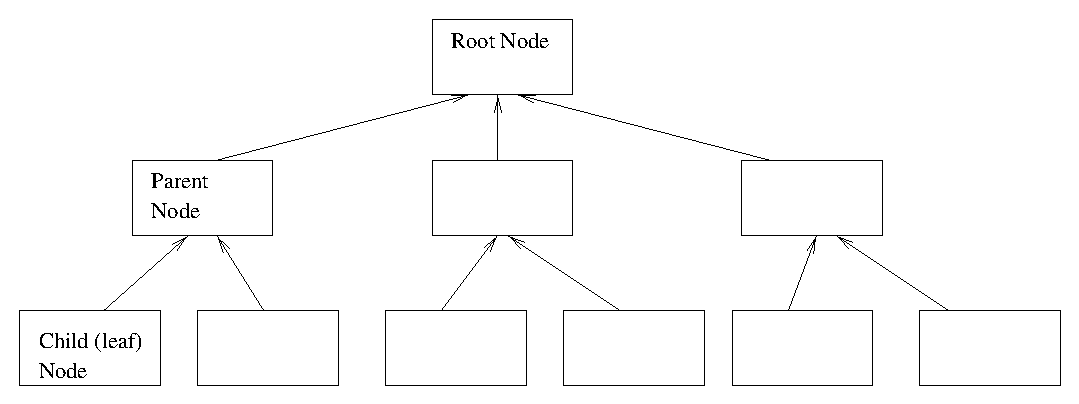
\includegraphics{figs/hier.eps}}}
%	\center \includegraphics[0\in,0\in][5\in,8\in]{figs/usage_table.eps} 
	\caption[Hierarchical Algorithm]{Hierarchical processor allocation
	algorithm: The parent of a node is a supervisor.  All work requests
	are given to the direct supervisor.  If a processor under that
	parent is free, the supervisor gives it to that processor.
	Otherwise, the process is handed to that supervisor's supervisor
	until a free processor is found or the root of the tree is reached.
	Upon reaching the root of the tree, a request is queued until a
	processor becomes available.}  \label{fig:hier}
\end{figure}

A hierarchical algorithm (see figure \ref{fig:hier}) for processor
allocation works as follows: All processors are set up in a virtual
hierarchy (tree structure), such that some processors are workers and others
are supervisors.  Supervisors also have supervisors until the root of the
tree is reached.  The way the algorithm works is as follows.

When a request for work is generated, that request is sent to the immediate
supervisor.  If the supervisor has enough free workers to perform the
request, then the supervisor allocates the work to those workers.  If not,
the supervisor sends the request to his supervisor.  This process continues
until a supervisor who receives the request has enough free processors to
allocate the work.  If the request reaches the root supervisor and no
processors (workers) are available, then the root supervisor holds the
request until a worker becomes available.

Fault tolerance in this approach can also be provided.  If a supervisor
fails, then a worker for that supervisor is promoted to the supervisor
position.


\subsection{A Microeconomic Algorithm \cite{econ}}

Another distributed approach to processor allocation is one based upon the
concepts of microeconomics.  This approach is modeled after an economy.
Competition sets prices for resources (e.g., the CPU).  Jobs compete for
resources by issuing bids and resource allocation is made through auctions.

In this approach resources and jobs are viewed as agents.  Each agent has a
goal and rules to follow in order to achieve its goal.  Each agent attempts
to achieve its goal without cooperating with any other agent.  Effective
global allocation of jobs is achieved indirectly through selfish competition
(Invisible Hand).

When a job enters the system, it is given an initial amount of money.
Whenever it migrates through the system it must pay to cross a link.  It
must also pay for CPU time.  Processors sell CPU time and communication
bandwidth, and they set their own prices.  A processor's goal is to maximize
revenue.  In order to get information on the prices of remote resources,
processors advertise on Bulletin Boards of adjacent processors.  Based upon
current pricing information, amount of money remaining, and resource
demands, jobs attempt to purchase resources and to be serviced.

Whenever a processor becomes idle, it holds an auction for resources.  If
local prices change a processor may send an advertisement to its neighbor
processors.


\subsection{Decentralized Load Sharing in Condor \cite{condor}}

A distributed system named Condor currently uses a decentralized load
sharing algorithm \cite{condor_load}.  Its algorithm is unique in two ways.
(1) A processor broadcasts its load information using a region-change
approach.  In other words, processor information is broadcast only when
there is a significant change and it is only broadcast to a select number of
workstations.  (2) Task collision, the situation where many jobs are sent to
a single station simultaneously, is avoided by using a preferred list
approach.

The preferred list is defined as follows: ``A workstation is the $k^{th}$
preferred workstation of one and only one other workstation, where $k$ is an
integer.''  and ``If workstation $i$ is the $k^{th}$ preferred node of
workstation $j$, then workstation $j$ is the $k^{th}$ preferred node of
workstation $i$.''  Using a preferred list, the probability of more than one
workstation sending their jobs to the same workstation is very low and
transferred tasks are evenly distributed.

A CPU is available for remote computation only if the keyboard is idle, the
CPU is idle, it can handle the job requirements, and no other remote task is
currently running on it.  In the implementation, these requirements are
translated to the following numbers: the average load $\leq 0.3$, the
keyboard is idle $> 15$ minutes, and no remote task is currently running.

A processor is chosen based upon its priority.  The priority of a
workstation is incremented by the number of individual users with tasks
queued on that workstation.  The priority is decremented with the number of
tasks submitted to that workstation and currently running (either remotely
or locally).  The workstation with the highest priority is contacted and
requested to run the job.  If swap space is sufficient, it accepts,
otherwise the request goes to the next highest priority processor.  If no
processor accepts the job, it runs locally.


\subsection{Theimer and Lantz Approaches \cite{idle_workstations}}

Theimer and Lantz offer two approaches for processor allocation.  One
approach is centralized and the other is distributed.  In the centralized
approach, clients periodically send status information to a central server,
and all remote execution requests go through that same server.  Instead of
all clients sending status information to the server and being included in
processor allocation decisions, only those clients with a load below a
certain threshold participate.  The group of machines that do send requests
to the server are known as host selection candidates.

The use of host selection candidates reduces the amount of network
communication considerably and allows the algorithm to scale well.  In
simulations, Theimer and Lantz showed that their centralized approach could
work well with up to 1600 machines in the system.  They also provided fault
tolerance in the following way:  At least $k$ entities monitor the
server to detect failure.  Whenever the server fails, a new instance of the
server is reconstructed by multi-casting a request for immediate state
update.  This approach to fault tolerance introduces a delay in service if a
failure does occur since server reconstruction takes time.

Another approach to fault tolerance is to use $k + 1$ replicas of the server
in order to survive $k$ failures.  Multi-casting provides a simple and cheap
way of updating multiple copies of the server.  

The second processor allocation approach offered by Theimer and Lantz is a
decentralized scheduler, which they claim to be less complex but also less
scalable than their centralized approach.  In their decentralized approach,
each client performs its own host selection (location policy).  Only those
clients needing to perform a host selection gather information from the
system.  When a client does collect information, it sends a request by
multi-casting a query to those machines containing idle resources.  How the
client knows which machines are idle was not addressed by Theimer and
Lantz.  

The client receives replies from all willing candidate machines and the
client selects the best candidate.  The problem encountered by this approach
is the large number of messages generated, $O(n^2)$ (where $n$ is the number
of machines), and the large number of replies received almost
simultaneously.  In order to cut down on network traffic, a client waits for
only the first $m$ replies, where $m$ is user definable.  Replying machines
place a weight on a random delay before sending their replies.  The weight
is determined by how good a candidate machine thinks it is for accepting a
remote execution request.  This approach gives non-optimal but good
selection as opposed to their centralized implementation.


The Theimer and Lantz approaches assume efficient broadcast and multi-cast
communication and that the cost of multi-casting to non-recipient machines is
negligible or none.  Theimer and Lantz also assume that nearly all of
the processes in their system are either short-lived or interactive.




\subsection{Random Probe Sets \cite{random_probe}}

Eager, Lazowska, and Zahorjan discuss a random probe set approach to
processor allocation.  Whenever a new job is created, the local machine load
is compared to some threshold.  If the local machine load is less than the
threshold, then the new job runs locally.  Otherwise, the task can be
forwarded to remote machines, up to some fixed number of forwards (in order
to prevent thrashing).  Remote servers are chosen by probing a small random
set of machines for load.  Surprisingly, this approach performs quite well
under simulation.

The goal of Eager, Lazowska, and Zahorjan was to achieve improved
performance in a distributed system with as little information as possible.
The two extremes for information gathering are no information gathering and
complete information gathering.  \cite{random_probe} chose to gather little
information by randomly probing a small set of machines whenever offloading
needed to occur.


\subsection{Stumm Approach \cite{stumm}}

The Stumm approach is based on server machines advertising their load,
rather than clients querying for load averages.  Advertising requires $O(n)$
messages, whereas querying generates $O(n^2)$ messages, where $n$ is the
number of machines in the systems.

However, hosts must always keep track of global state information.  New
hosts must wait for update messages from other machines before they can
offload jobs.

\subsection{Distributed Load Balancing using a Local Process Queue \cite{Hac}}

Hac and Jin perform dynamic load balancing using a decentralized approach.
Lightly loaded processors search for heavily loaded processors.  Each
processor dynamically calculates a threshold $T = trunc ( \frac{\mbox{Number
of Active Processes on all remote machines}}{\mbox{Number of remote
processors}} )$.  Each processor also has a value $C = \mbox{maximum number
of active processes allowed}$.  This prevents the system from being
overloaded.

The algorithm consists of three routines: The Local Process Queue Routine
monitors for new jobs.  When a new job is created, it is placed on the end
of the local job queue if the $\mbox{Number of active processes} > C$.
Otherwise, the job executes immediately.

The Local Monitor Routine runs whenever the local process queue becomes
empty.  It searches for the most heavily loaded machine (the one with the
longest queue) and obtains the first job from that local process queue.
Semaphores are provided to prevent two processors from obtaining the same
job simultaneously.

The Distributed Monitor Routine broadcasts load information to other
machines in the system.  If a processor becomes saturated (i.e.,
$\mbox{Number of jobs in local process queue} > C$), it can suspend the
distributed monitor routine until its load falls.

This system was tested under simulation using three types of processes:
CPU-intensive, I/O-intensive, and CPU-I/O-intensive.  Performance was
measured by mean response time compared to the number of processors in the
system.

\subsection{Receiver Initiated Distributed Heuristic Algorithm \cite{Tanenbaum}}

In this approach, whenever a workstation determines that it needs more work
(e.g., its load average is below some threshold), it advertises that it
needs more work.  To do so, it selects another machine within the \ds at
random and then requests work from that machine.  If the machine gives it
work, then the requesting workstation performs it.  Otherwise, it picks
another machine at random from which to request work.

The requesting workstation continues to request work until it finds it or
until it polls $n$ machines.  After polling these $n$ machines, it stops
polling for a certain amount of time or until it gets more work locally.


\subsection{Dynamic Scheduling in Shared-Memory Multiprocessors
\cite{shared_queue}}

A common approach to load balancing (scheduling) in a shared-memory
environment is to place all new jobs in a shared queue.  Whenever a
processor becomes idle, it allocates work to itself from the shared queue.
According to Hamidzadeh and Lilja in \cite{shared_queue}, this approach
requires a lot of overhead in accessing the shared queue and directly
increases the overall execution time.  They offer an alternative approach.

Hamidzadeh and Lilja try to minimize memory delay in process execution by
considering locality of memory references.  The name of their approach is
SADS (Self Adjusting Dynamic Scheduling).  One processor performs a branch
and bound algorithm to compute scheduling based on loads of other processors
and memory locality information.  SADS searches through all partial and
complete searches using a heuristic.  There is also a depth-bounded version
of SADS.  

When SADS completes its dynamic scheduling, it places jobs in local queues
of processors.  To improve performance and reduce wait time, SADS performs
its partial scheduling in repeated scheduling periods, self-adjusting the
amount of time allocated to each scheduling period to minimize idle times.




%%%%%%%%%%%%%%%%%%%%%%%%%%%%%%%%%%%%%%%%%%
%%
%%  Objectives
%%
%%%%%%%%%%%%%%%%%%%%%%%%%%%%%%%%%%%%%%%%%%





\chapter{Objectives and Criteria}
\label{obj_criteria}

\section{Objective}

Given a collection of processors, each of which can receive external job
requests, fair processor allocation should be performed for newly incoming
jobs.  In the case of dynamic process migration, fair processor allocation
should occur during the lifetime of processes.  Since the goal of the
algorithm is to load balance, the unfairness at time $t$ can be measured by
the maximum difference in jobs between two processors.  The performance of
an allocation method over a time period can be measured by the average
unfairness over that time period.

The goal of this research was to design and implement three processor
allocation algorithms, one centralized and two distributed.  Each algorithm
is explained in detail in section \ref{algorithms}.  Three environments were
implemented for these algorithms: simulation, quasi-simulation, and a full
implementation.  Performance criteria and test cases were developed and are
used to compare the three algorithms and the three environments.




\section{Algorithms}
\label{algorithms}


\subsection{Token based Algorithm}

\begin{figure}
	\resizebox{\textwidth}{!}
	{\rotatebox{360}{
	\includegraphics{figs/token.eps}}}
%	\center \includegraphics[0\in,0\in][5\in,8\in]{figs/usage_table.eps} 
	\caption[Token based Algorithm]{Token based processor allocation
	algorithm: A usage table containing current load and memory usage
	information in a token circulates around a logical ring of
	processors, updating information as it circulates.}
	\label{fig:token}
\end{figure}


At startup, a logical ring is constructed, where each node in the ring
represents a processor in the distributed system.  A coordinator is then
elected using an election algorithm.  A single packet (the token) is then
transmitted by the coordinator with an entry for each processor in the
system.  The entry contains the following information for each machine: load
and amount of free memory.

Each time a machine receives the token, it does the following things:

\begin{enumerate}
  \item The machine updates the token's usage table with its current load
  and amount of free memory.

  \item If the machine wants to offload a process, it picks the machine with
  the lowest load that has enough free memory, and migrates the
  process to that machine.  

  \item The machine forwards the token to the next machine in the logical
  ring. 
\end{enumerate}


For fault tolerance, ring and token management procedures are implemented.
A coordinator is elected at startup.  The coordinator monitors for lost and
duplicate token.  If a token is duplicated, the coordinator removes one of
the tokens from the ring.  If a token is lost, the coordinator generates a
new token.  Other members in the ring monitor for coordinator failure. If
the coordinator fails, then a new coordinator is elected.

When a new job is introduced to the system, the originating machine sets a
timeout (adjustable by the user) for when the process is to be accepted.  If
the process has not been accepted by the timeout, then the originating
machine broadcasts a message to other members of the ring to see if they are
alive.  If a machine does not respond, then it is assumed to have failed and
it is removed from the ring.  The process can be resubmitted to the system,
ensuring at least once execution semantics.  See figure \ref{fig:token}.



\subsection{Distributed Q-learning Algorithm}

\begin{figure}
	\resizebox{\textwidth}{!}
	{\rotatebox{360}
	{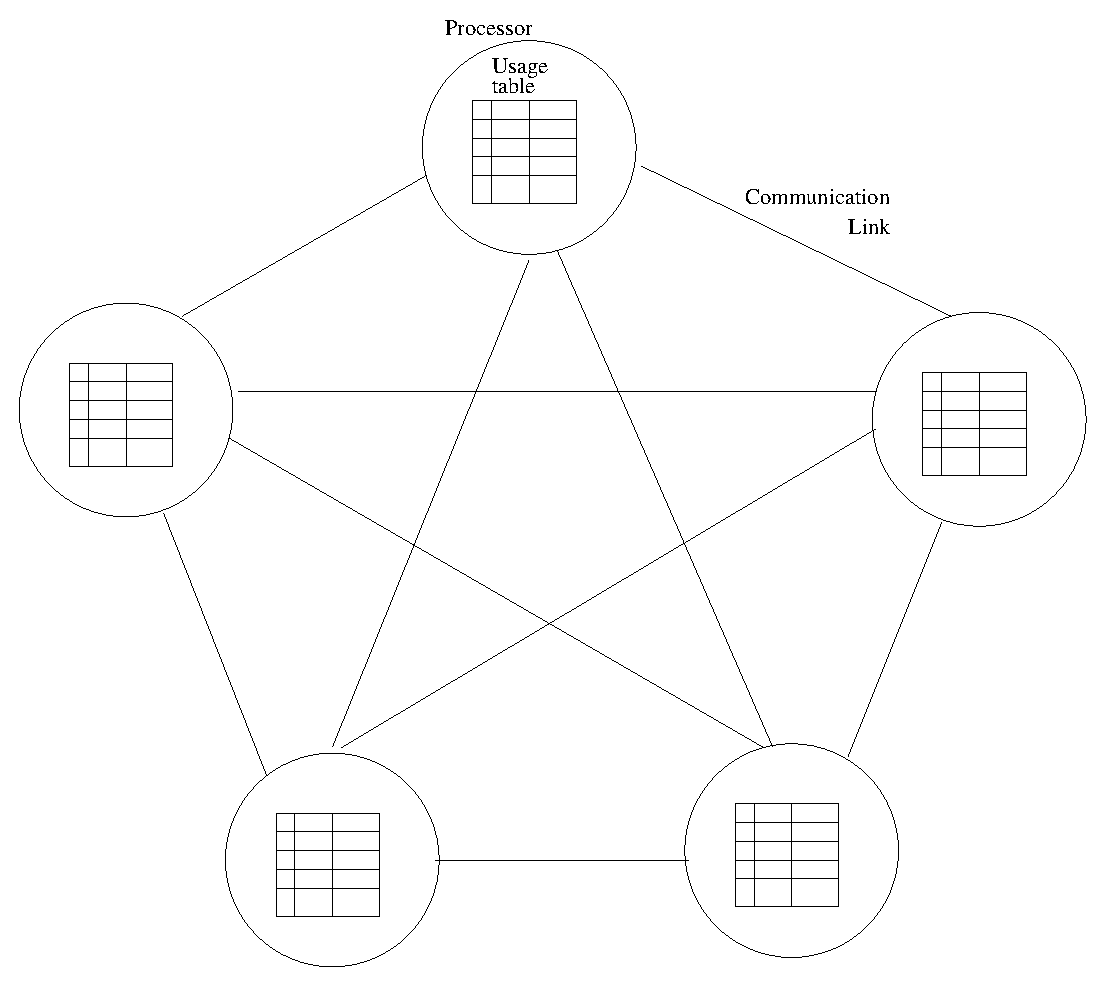
\includegraphics{figs/random-dpa.eps}}}
%	\center \includegraphics[0\in,0\in][5\in,8\in]{figs/usage_table.eps} 
	\caption[Distributed Q-learning Algorithm]{Distributed Q-learning
	processor allocation algorithm.  Each processor maintains a usage
	table.  Based upon this usage table, a processor can offload a
	process to any other processor in the system.}
	\label{fig:random}
\end{figure}


Each machine maintains a table comprised of values reflecting the last known
load on each machine.  Initially, all values are zero (neutral).  When a new
job is introduced to a processor, that processor allocates the job to some
processor in the system, perhaps itself.  This choice is based on the table
most of the time and made randomly the rest of the time (defined by
parameter $p$, which is an integer between 0 and 100).  Parameter $p$ is
used as a percentage.  For example, if parameter $p$ is $25$, then
processor selection will be made randomly $25\%$ of the time and based upon
a table the other $75\%$ of the time.

The table is updated in the following way: When processor $A$ chooses to
give a job to processor $B$, $A$ sends a request to $B$, which includes
$A's$ current load.  $B$ updates its table using this information and
decides whether to accept the job or forward the request to another machine.
Ultimately, some machine $C$ accepts the request and obtains the job from
$A$.  

Each machine ($A$ through $C$) updates its usage table using load information
passed to it in the request message, which is appended to the request as it
is forwarded to each machine.  A naive update rule is simply to replace old
data with new data.  However, a better approach might be to use weighted
average of the old and new data, perhaps incorporating the age of the old
data.  

The only way a job could bounce around the system indefinitely is for new
jobs to be introduced to the system faster than the system can send messages
back and forth between machines.  This is is highly unlikely, thus in
practice there is no indefinite postponement of jobs, although theoretically
it is possible. To ensure that indefinite postponement does not occur, a hop
count limit (implemented as the size of the distributed system + 1) is
imposed.  A machine receiving a request message with the hop count limit
surpassed is forced to accept the process.


For fault tolerance, machines can be dynamically added and removed from the
system.  The system also detects failures of processors by using timeouts on
process creation requests.  When a new job is introduced to the system, the
originating machine sets a timeout (adjustable by the user) for when the
process has been accepted.  If the process has not been accepted by the
timeout, then the originating machine broadcasts a message to other members
of the system to see if they are alive.  If a machine does not respond, then
it is assumed to have failed and it is removed from the local usage table.
The process can be resubmitted to the system.  This ensures at least once
execution semantics.  See figure \ref{fig:random}.


\subsection{Centralized Algorithm}

For comparison reasons, a modified version of the Mutka/Livny up-down
algorithm was implemented.  In this centralized algorithm, all process
creation requests go through a single machine, although they can still
originate anywhere.  When a process is offloaded to a machine by the
coordinator, that machine must return its reply that it has accepted the
process.  The same is true when the process finishes.  Hence, the
coordinator always knows (within time $\epsilon$, defined to be the amount
of time for a client to respond to the coordinator) when a remote machine is
executing a process.

In the Mutka/Livny up-down algorithm, processes wait until a processor
becomes free before they start executing.  In this modified version, there
is no notion of a processor being busy.  All processes are offloaded
immediately when they are created.  Therefore, a processor's usage value
does not get decremented for waiting-to-run processes.  Hence, usage values
are always zero or higher.

Whenever, a process is offloaded, the coordinator checks its usage table to
determine which processor it deems to have the lowest load.  The process is
then migrated to that processor for execution.  While the process is
running, the processor running it accumulates a usage point every $m$
seconds.  If a processor is running $n$ processes, it accumulates $n$ usage
points every $m$ seconds.  While a processor remains idle, its usage value
is decremented by $1$ usage point every $m$ seconds until the usage value
reaches zero.


\section{Criteria}
\label{sec:criteria}

In general, distributed systems can be compared using the following
criteria \cite{Tanenbaum}.  Distributed processor allocation is no
exception.


\begin{itemize}
	
  \item Transparency

	The distributed system should provide services such that the user is
	unaware of where within the system that the services take place.
	The system should function, at least from the user's perspective, as
	a single unit. 


  \item Flexibility

	The distributed system should be designed in such a way that it is
	easily changeable and customizable.

  \item Reliability

	The distributed system should provide consistency and should
	function even in the presence of failures when possible.  In other
	words the distributed system should be fault tolerant.  When
	possible, failures should go unnoticed by the user.

  \item Performance

	The distributed system should provide a reasonable and consistent
	response time to users and in general the system should provide a
	level of performance not less than that of a stand-alone machine.
	In other words, the distributed system should not penalize
	performance, and when possible it should enhance it.

	\cite{Casavant} defines performance of a distributed algorithm as
the ``\dots degree to which an algorithm achieves its global objective.''
Efficiency is described as the ``\dots measure of the costs associated with
[the] level of goal achievement.''

  \item Scalability

	The design of a distributed system should be such that it functions
	appropriately and efficiently no matter how many machines comprise
	it.  

  \item Security

	The distributed system should prevent access to the system,
	including its processes, data, and services, from unauthorized
	users.  Furthermore, individual users should be protected from other
	users in the same system.

\end{itemize}


\subsection{Quantification of Criteria}

In order to effectively compare and contrast algorithms, it is useful to
quantify criteria.  In this way algorithms can be compared using numbers and
statistics rather than just words.

Several measurable statistics come to mind when measuring the
\textbf{performance} of a processor allocation algorithm:

\begin{itemize}
	\item Maximizing CPU utilization -- the comparison of the load
	averages of all processors over time.

        \item Minimizing response time -- the time elapse from process
        creation to process execution.

        \item Minimizing total elapsed time a process requires to finish -- 
        the time elapse from process creation to process termination.

	\item CPU overhead -- a ratio of the amount of CPU time used by the
	processor allocation algorithm to the total amount of CPU time
	available.

	\item Network bandwidth overhead -- a ratio of the amount of
	communication required by the processor allocation algorithm to the
	total network bandwidth.

	\item \cite{preempt} states the goal of its scheduling policy is to
meet users' performance expectations, which is centered on quality of
service provided to jobs a user starts.  Two measurable criteria used in
this approach are response time and response ratio.  Response time is
defined to be the total amount of time a process resides in the system,
whereas response ratio is the response time per unit of service.

\end{itemize}

\emph{Scalability} can be measured by comparing the results of performance
measurements of the algorithms running variable sizes of distributed
systems.  A good way to quantify scalability is to show total execution time
of $n$ processes in a system with $m$ processors.

\emph{Fault Tolerance} can be determined by introducing failures into the
distributed and accessing whether the system continues to perform.  If so,
then how the performance level is effected is an interesting statistic.

\emph{Flexibility} is not something that can easily be measured and hence a
descriptive explanation of the features that make an algorithm flexible will
need to be discussed, such a modularity, ease of use, etc.

\emph{Transparency} also is difficult to measure, so again a descriptive
explanation of why and how an algorithm is transparent will be given.

\emph{Security} is not addressed in this thesis.


\subsection{Metrics}

\label{sec:metrics}

Metrics are classified into three categories: message statistics, processor
statistics, and process statistics.  Message statistics include the number
of each type of message generated and the sizes of each type of message
generated.  Averages and standard deviations can be computed for these.

Process statistics include the response time (time from creation to initial
execution), the hop count of request messages for a process before it is
accepted, and the total time a process resides in the system.  For
scalability comparisons, the total execution time of $n$ processes in a
system with $m$ processors is also shown.

Processor statistics show the load average of processors over time as well
as the average load and standard deviation.

There are a large number of other statistics that can be tracked and used to
compare processor allocation algorithms.  Due to the human inability to
compare an overwhelming amount of information, a small set of statistics is
preferable to a large set.  However, it is important that this small set of
statistics represents the major aspects of performance comparisons.



\section{Issues}


\subsection{Location policy}

Load alone may not be enough to determine the best processor on which to
offload a process.  From a user point of view, a distributed system should
offer better or equal performance as compared to a stand-alone machine.
Hence, criteria such as time delay between process creation and initial
execution is important.  Items that would effect this include hop count of
messages in the network, whether a binary needs to be migrated across the
network, etc.

Another important variable to check when offloading processes is the amount
of free physical memory.  If a machine does not have enough free memory to
run a new process then it would be pointless to try running it there.
However, memory requirements of a a process are rarely known before runtime.
Still, if a machine has little free physical memory, performance might be
effected due to swapping.  Hence, many factors other than load might need to
be taken into account when determining the best machine on which to offload
a process and when comparing the performance of processor allocation
algorithms.

Location policy depends highly upon the type of job being transferred.  For
CPU-intensive job, load alone is a good indicator.  However, for
disk-intensive jobs, the number of blocks read and written, and the location
of file servers for files opened by a process are a large determinant of
location policy.


\subsection{Selection policy}

The threshold of the selection policy is the point at which migration or
placement begins.  Threshold selection can be either dynamic or
static. \cite{gradient} discusses a dynamic approach to threshold
selection.  The algorithms implemented here use a static approach as
discussed in section \ref{threshold}.


\subsection{Preemption versus non-preemption}

According to \cite{preempt}, preemptive scheduling can increase the
performance of a distributed system.  However, preemption is difficult to
implement because process state must be captured and transferred across the
network in order for a process to resume where it was preempted.  Also, one
must determine when to it is more efficient to migrate an already running
process rather than to let it finish execution where it currently runs.

Logic dictates there are at least several factors to use in determining when
to preempt and then to migrate a process.  These include (1) The load
average on the current machine (2) The load average on a potential new host
(3) The amount of time, CPU overhead, and network overhead required to
preempt and migrate the process across the network.  Since the goal of
migration is to minimize the overall time from process creation to
completion, all three factors must be taken into account.

It certainly makes little sense to migrate a process from a machine with a
load average of $4$ to a machine with a load average of $3$, especially
since a new job could be started on the more lightly loaded machine while
the preempted process is migrating.  Also, the load average on the current
machine could fall by the time the preempted process migrates since
another process could complete in the meantime.  Ultimately, there must be a
significant difference in load average between the two machines in order for
migration to produce better results.


\subsection{Testing}

Testing is a very difficult task and there are many issues associated with
it.  First of all, there are many variables to take into account when
testing.  Not all combination of variables can realistically be tested.
Hence, a subset of important variable combinations must be used to
demonstrate the main aspects of each system.  Since a fair amount of
randomness exists in each algorithm, many test runs need to be performed to
get statistically meaningful data.




%%%%%%%%%%%%%%%%%%%%%%%%%%%%%%%%%%%%%%%%%%
%%
%%  Implementation
%%
%%%%%%%%%%%%%%%%%%%%%%%%%%%%%%%%%%%%%%%%%%



\chapter{Implementation}

The three algorithms were implemented using kali-scheme, a distributed
implementation of scheme48 \cite{kali}.  Using kali-scheme processors can be
simulated using threads in a single \UNIX process, several \UNIX processes on
the same physical machine, or several \UNIX processes on multiple physical
machines.

\section{Environment}

For testing purposes and comparison reasons, three testing environments for
of all three algorithms were developed.  The first environment is a complete
simulation; the second is a quasi-simulation; and the third is a full
implementation.

In the complete simulation, processes and processors are modeled using
threads in a single process.  The load and memory requirements of each job
are specified when the job is created.  This allows the user to control
the load of jobs introduced into the system for test purposes.  The load
average of a processor is simply the sum of the loads of all jobs currently
running on that processor.  The amount of memory used is the sum of the
memory requirements of all jobs currently executing on a particular
processor, and the amount of the free memory is the total amount of memory
minus the amount of memory used.

Processors are modeled as objects in the object-oriented style and they
communicate with one another by sending messages.  Jobs are modeled as
threads.  Whenever a new job is allocated a processor $A$, the load and
memory of processor $A$ are adjusted and the thread runs.  When the job
finishes, the load and memory are adjusted again.

Processes in the simulated environment do nothing but sleep for a period
time specified by the user.  Therefore, simulated processes contributed no
actual load to the system.

In the quasi-simulation, processes and processors are still modeled as
threads, but each processor object actually resides on a different physical
machine.  Hence system state information is actually communicated across the
network and jobs actually run on different physical machines.  Load averages
and memory requirements are not given by the user when jobs are created but
rather they are calculated by the system.  A thread load calculation was
implemented for kali-scheme, which is based upon how the Linux operating
system computes load averages of processes.

Processes in the quasi-simulation are scheme threads that perform some kind
of computation or input/output.  They, therefore, contribute load to the
scheme process.

Finally, for the full implementation, jobs are not modeled as threads but
are real \UNIX processes, forked and executed by the system.  Real load
averages from the OS are obtained for state information.  While processors
are still modeled using threads within the kali-scheme processes, this is
simply for communication and information tracking purposes.  Each processor
thread in kali-scheme runs on a distinct physical processor since each
processor thread resides on a different physical machine.  This
implementation uses real processors, real processes, real load averages,
real memory requirements, real network communication, and real faults.
Preemption was not implemented for this approach in order to reduce
complexity.

\section{System Architecture}

The design of this system is separated into several entities: processors,
processes, communications, logging and statistics generation, each of which
can be divided into its constituent parts.

Processors:
\begin{itemize} 
	\item Processor scheduler
	\item Load average calculator thread
\end{itemize}

Processes:
\begin{itemize}
	\item Simulated processes with varying load contributions and
	execution times
	\item Scheme threads for the quasi-simulation that perform actual
	computations 
	\item Real \UNIX processes that perform computation
\end{itemize}


Communications:
\begin{itemize}
	\item Network daemons
	\item Messages: token, process creation, etc.
	\item Ring-procedures (for token-based algorithm)
	\item Token-procedures (for token-based algorithm)
\end{itemize}


Logging:
\begin{itemize}
	\item Processor logging thread
	\item Scheme-readable format
	\item Human-readable format
\end{itemize}

Statistics generation:
\begin{itemize}
	\item x-y plots of processor load average over time
	\item x-y plot of average processor load over time
	\item x-y plot of standard deviation of processor loads over time
	\item x-y plot of maximum unfairness of processor loads over time
	\item Process response and execution times
	\item Hop counts processor request messages
	\item Counts of message types produced by the system
\end{itemize}



\section{Load Average Computation}

Load average in the quasi-simulation and in the real implementation is
implemented in the following way: Load average is calculated over the past
1, 5, and 15 minutes using an exponential decay algorithm.  This gives a
weighted average of the current load with previous loads (of 1, 5, and 15
minutes).  The current load is defined to be the length of the ready queue.
The weight of the current load in calculating the load average over the past
minute is $1 - e^{interval - 60}$, whereas the weight of the previous load
is $e^{interval - 60}$, where \emph{interval} is the frequency (in seconds)
at which the load is updated.  This algorithm was adapted from the Linux
kernel implementation coded by Linus Torvalds and appears in figure
\ref{fig:load_avg_alg}. 

\begin{figure}
\label{fig:load_avg_alg}
\caption{Load Average Algorithm: Calculates the load average every 5 seconds
for the past 1, 5, and 15 minutes.}

\begin{verbatim}

(define calc-load

  ;; load is a vector of three elements, containing the load average over
  ;; the last 1, 5, and 15 minutes respectively.
  ;; ready-Q is the ready-Q of the scheduler.

  (lambda (load ready-Q)
    (let*
        ((interval 5000)                ; 5 sec
         (exp-1 (exp (* -1 (/ (/ interval 1000) 60))))
         (exp-5 (exp (* -1 (/ (/ interval 1000) 300))))
         (exp-15 (exp (* -1 (/ (/ interval 1000) 900)))))
      (letrec 
          ((calculate
            (lambda (which exp-n num-tasks)
              (vector-set! load which
                           (+ (* (vector-ref load which) exp-n)
                              (* num-tasks (- 1 exp-n))))))
           
           (update-load
            (lambda ()
              (let
                  ((num-tasks (queue-length ready-Q)))
                (calculate 0 exp-1 num-tasks)
                (calculate 1 exp-5 num-tasks)
                (calculate 2 exp-15 num-tasks)
                (sleep interval)        ; recalc load every interval
                (update-load)))))
        (update-load)))))

\end{verbatim}

\end{figure}


\section{Fault tolerance}

Processors can be dynamically added and removed from the system.  When a
processor is added to the system, it broadcasts its state.  In the
centralized algorithm, it sends a message only to the server.  In the same
way, when a machine properly shuts down, it sends a message to the server or
it broadcasts it to the system.  For the distributed algorithms, processor
addition and removal requires $O(n)$ messages whereas the centralized
algorithm requires only $O(1)$ messages, where $n$ is the number of machines
in the system.

The token-based algorithm uses the fault tolerance procedures of a generic
token algorithm, such as coordinator election in the presence of coordinator
failure, token generation whenever a token is lost, and token removal
whenever multiple tokens are present.

Whenever a process is created, the machine on which it is created must
ensure that the process begins execution on some remote machine.  This is
accomplished via a reply to the originating machine whenever the process is
accepted.  The originating machine simply uses a timeout to ensure it
receives this response.  If not, it broadcasts to all processors it knows
about.  If it does not receive a reply from a particular processor within a
fixed amount of time, that processor is removed from its usage table.  The
originating machine can also resend the remote-execution request.  This
ensures at least once execution semantics.  This approach provides fault
tolerance for process execution and for processor failures.

Instead of timing out on every message, timeouts need only occur to ensure
processes are accepted.  This considerably reduces the amount of state
information and the amount of messages generated in order to incorporate
fault tolerance into the algorithms.  Essentially, the only message increase
occurs when an accept message is not received before the timeout.  Then
$O(n)$ messages are produced, where $n$ is the the number of processors in
the system.  However, this occurs very infrequently -- only when a processor
is assumed to have failed.  Otherwise, the system experiences no increase in
messages.  In the centralized algorithm, only $O(1)$ messages are produced
when a timeout occurs.


\section{Messaging}

Messaging is currently provided by a centralized mail server, but can easily
be made distributed without effecting the rest of the system, since the mail
system is modular.

For group messaging, FIFO broadcast semantics is provided by the mail
system.  \definition{FIFO Broadcast}{All messages sent by a single process
will be received in that same order by all recipients. In other words, if
processor $A$ sends messages $1$ and $2$ to processors $B$ and $C$, then
both $B$ and $C$ will receive the messages from $A$ in the same order they
were sent. This scheme allows $B$ to receive both messages $1$ and $2$
before $C$ receives any messages.}{def:fifo_broadcast}

In the simulated token-based algorithm, the token is sent between processors
in the logical ring by sending a message to the processor object.  In the
distributed implementation, since each processor object resides on distinct
physical machines, an actual network packet is be generated for this token.

Several types of messages exist in the system:

\begin{itemize}
	\item processor-add: A new processor is available for remote
		 computation.
	\item processor-remove: A processor is no longer available for
		 remote computation.
	\item processor-shutdown: Makes a processor shutdown.
	\item process-create: A process creation request
	\item process-accept: Message notifying owner of a process that it
		 has been accepted.
	\item process-done:  Message notifying owner of a process that it
		 has completed computation.
	\item request: Message requesting a machine to accept a process.
		 In the distributed Q-learning algorithm, this message has
		 load information piggybacked onto it.
	\item alive?: Message asking a remote machine to respond.  Used for
		 fault tolerance to ensure a remote processor is still
		 available in case a process request has timed out.
	\item alive!: Message responding to an alive? message.  Indicates
		 that a machine is still available for remote computation.
	\item token:  Used only in the token-based algorithm, this type of
		 message transmits the usage table around the logical ring.
	\item update: Used only in the distributed Q-learning algorithm,
		 this message is sent to the owning machine when a process
		 has been running remotely for $5$ seconds.  This allows the
		 load to be affected by the new process.
	\item log: Used for information gathering, this type of message
		 requests that a processor log its current load information
		 to a log file.
\end{itemize}



\section{Processes}

Three types of jobs were used to test the system: 

    \begin{itemize}
	\item CPU-intensive
	\begin{itemize}
		\item Simulation: scheme thread sleeps for 35 seconds and
	contributes a load of 1 to the system load.
		\item Quasi-simulation: interpreted scheme thread repeats math
	multiplication $5,000,000$ times.
		\item Full implementation: \UNIX process written in C
	repeats math multiplication $150,000,000$ times.
	\end{itemize}

	
	\item Disk intensive
	\begin{itemize}
		\item Simulation: scheme thread sleeps for 18 seconds and
	contributes a load of 0.6 to the system.
		\item Quasi-simulation: interpreted scheme thread writes 
	250,000	characters to to file.
		\item Full implementation: \UNIX process written in C
	writes 3,000,000 characters to a file.
	\end{itemize}


	\item Highly interactive: Job that sleeps, accesses memory, and 
	loops $n$ times.  The process is designed this way instead of having
	user interaction so that the issues of console redirection over the
	network are avoided.
	\begin{itemize}
		\item Simulation: scheme thread sleeps for 10 seconds and
    contributes a load of 0.01 to the system.
		\item Quasi-simulation: interpreted scheme thread sleeps for
    3 seconds, performs 100 memory operations and loops 6 times.
		\item Full implementation: \UNIX process written in C sleeps
    for 3 seconds, performs a memory operation and loops 6 times.
	\end{itemize}

    \end{itemize}


\section{Randomness}

For the source of randomness in the distributed Q-learning algorithm, a
random number generator distributed with kali-scheme was used.


\section{Process Migration}

Each process maintains a migration count in its process control block.  The
migration count of a process gets incremented by $1$ each time a process
migrates to a new machine.

The selection algorithm used is simple.  The first process in the process
table with the lowest migration count gets selected for migration.  The
process migration algorithm runs every $n$ seconds.  If the load is over a
certain threshold and there is a more lightly loaded machine in the (by a
certain threshold), then a process is migrated, and its migration count is
incremented. 

This approach prevents indefinite postponement of processes by ensuring that
a process migrated once is not migrated again until every other process on
that machine migrates at least once.

\section{User controlled variables}
\label{user-config}

The following variables are controllable by the user:

\begin{itemize}
	\item environment: full implementation, quasi-simulation, or
	simulation. 

	\item process-migration-load-threshold: If a processor's load is
	greater this threshold, the migrator thread will migrate a process
	to a more lightly loaded processor

	\item process-migration-load-diff-threshold: In order for a
	processor to migrate a process the difference between its load and
	the minimum loaded processor must be at least this 

	\item process-migration-interval: How often the process migration
	procedure runs. 

	\item timeout-wait-period: Amount of time a processor waits to
	receive an ACCEPT message for an offloaded process before invoking
	fault tolerance procedures 

	\item processor-timeout: Amount of time a processor waits to receive
	an ALIVE reply from another processor before invoking fault
	tolerance procedures 

	\item migrate-processes: Should process migration occur?

	\item token-threshold: How often should the coordinator check to see
	if it has seen the token? 

	\item coordinator-threshold: How often should machines in the system
	check to see if the coordinator is alive?

	\item parameter-p: Used only the distributed Q-learning algorithm,
	this value is the percentage of time that a processor is chosen at
	random for offloading a process.

	\item usage-table-update-interval: Used only in the centralized
	algorithm, this value is the how often the usage table values are
	adjusted on the server.
\end{itemize}



\section{Logging and Statistics}


For statistical purposes, each processor logs its load every $n$ seconds.
This log is centralized such that all processors log to the same file.  A
lock on the file prevents multiple processors from writing to the log
simultaneously.  In the distributed implementations, a processor calls this
logging function as a remote procedure and hence all logging takes place on
a single machine.  Since the logging function runs on only one machine, a
single clock time stamps all log messages.  Therefore, clock synchronization
is not required in order to correctly interpret the log data.

The following statistics are tracked as the system runs:

\begin{itemize}
	\item Load average of processors over time

	\item Memory usage of processors over time. 

	\item Maximum unfairness ($max\_load - min\_load$) of processors
	over time. 

	\item Average processor load over time

	\item Standard deviation of processor load from the average over
	time.

	\item Response time: time elapse from process creation to process
	execution.

	\item Total elapsed time: time elapse from process creation to
	process termination.

	\item Average number of hop counts for all processor request
	messages.

	\item Number of local jobs and number of remote jobs for each
	processor over time.

\end{itemize}

When the distributed system is shutdown by the user, the log file is
converted to a human-readable format, and \texttt{gnuplot} data files are
automatically generated.  The \texttt{gnuplot} data includes the load
average of each processor over time, the maximum unfairness among processors
over time, and the the standard deviation of processor loads from the
average of all processor loads over time.

The data files generated for \texttt{gnuplot} were converted to x-y graphs
and are contained in appendix \ref{app:test-cases}.  Each chart shows load
(y-axis) versus time in milliseconds (x-axis).  In the load average graphs,
each line represents a different processor in the system, and one of the
lines represents the average load of all processors in the system.

The other data generated for comparison purposed include (1) the response
time and execution times for every process, (2) hop count data for request
messages, and (3) counts for each type of message generated during system
execution.  Samples of this data is contained appendix \ref{app:test-cases}.

\section{Selection policy}

For new processes, the selection policy is simple, all new jobs are
offloaded if a lower loaded machine exists.  For process migration, the
policy is to pick the process with the lowest migration count.  The system
was designed with CPU-intensive jobs in mind, so using the process with the
least migration count avoids choosing the same job time and again to be
migrated.  Otherwise, a job could be indefinitely postponed.

\section{Transfer policy}

The transfer policy is invoked every time a job is created.  The transfer
policy also runs every $n$ seconds to check for preemptive migration.  For
preemptive process migration, the system checks to see if its load is above
some threshold.  If so, and another machine has a lighter load (within some
threshold), then selection and transfer algorithms are invoked.  The
thresholds and $n$ are all user adjustable.

\section{Location policy}


Figure \ref{fig:selection_alg} shows an algorithm useful for processor
selection (location policy).  The actual algorithm used is a scaled-down
version that incorporates only load average as a factor.  So it is most
useful for cpu-intensive jobs.

\begin{figure}
\label{fig:selection_alg}

\begin{verbatim}

PROCEDURE calculate_priority BODY
   FOREACH processor in processor_list DO
       processor.priority <- ld_avg_wt * processor.load_avg +
                             mem_wt * processor.free_memory +
                             speed_wt * processor.speed
   OD
ENDPROC



FUNCT find_best_processor returns processor BODY
  IF (local_load < threshold)
  THEN
       return (LOCAL_PROCESSOR)
  ELSE
       filter (processor_list, processor_architecture_for_this_process)
       filter (processor_list, memory_requirements_for_process)
       calculate_priority (processor_list)
       best_processor <- minimum (processor_list, priority)

       return (best_processor)
  FI
ENDFUNCT


\end{verbatim}
\caption{Processor selection algorithm}


%\begin{programbox}

%\PROC calculate_priority \BODY
%   \FOREACH processor in processor_list \DO
%	processor.priority <- ld_avg_wt * processor.load_avg +
%				mem_wt * processor.free_memory +
%				speed_wt * processor.speed
%   \OD
%\ENDPROC

%\\

%\FUNCT find_best_processor returns processor \BODY
%  \IF (local_load < threshold)
%  \THEN
%	return (LOCAL_PROCESSOR)
%  \ELSE
%	filter (processor_list, processor_architecture_for_this_process)
%	filter (processor_list, memory_requirements_for_process)
%	calculate_priority (processor_list)
%	best_processor <- minimum (processor_list, priority)

%	return (best_processor)
%  \FI
%\ENDFUNCT

%\end{Programbox}

\end{figure}


This location policy algorithm is designed for CPU-intensive processes.



\section{Placement and Migration Thresholds}
\label{threshold}

The placement and migration thresholds are both static and user adjustable.
The placement threshold used for testing purposes was $0.0$.  The migration
threshold was $4.0$ and the load difference threshold was $3.0$.  Therefore,
in order to migrate a process, a processor must have a load average of at
least $4.0$ and there must be at least a difference of at least $3.0$
between it and the lowest loaded processor.  All new jobs can potentially be
offloaded.

The reason a load difference of 3 was used is because any less of a load
difference does not justify the overhead involved in transferring the
process and its state information to a remote machine.  Also, the migration
of an already running job must significantly improve its chances of gaining
processor time.

These placement and migration thresholds are arbitrary and more testing and
analysis needs to be performed for better thresholds.  Migration was not
implemented for the Centralized algorithm since individual machines have no
global knowledge, and therefore cannot compare their own load against
another load.


%%%%%%%%%%%%%%%%%%%%%%%%%%%%%%%%%%%%%%%%%%
%%
%%  Testing and Results
%%
%%%%%%%%%%%%%%%%%%%%%%%%%%%%%%%%%%%%%%%%%%


\chapter{Testing and Results}

Since the implementation of the processor allocation algorithms is very
flexible, there are many user-controlled variables.  Because of these
variables and because randomness exists in the systems, test cases need to
be designed in order to compare the performance of the algorithms.  In order
to further compensate for the randomness factor, several runs of each test
case are necessary.

\section{System Variables}

The following values can be changed while testing any of the processor
allocation algorithms.

\begin{itemize}

	\item \textbf{Number of processors in system}.  This can be one or more
	processors.  In the simulation the upper bound is limited by the
	number of threads that kali-scheme can handle, which depends mostly
	on the amount of memory available.  Through experimentation, 
	kali-scheme can handle thousands of threads simultaneously on a
	Sparc 5 box with 32 MB of RAM.  In the quasi-simulation, one is
	limited by the number of kali-scheme processes one can run
	simultaneously.  In the full implementation, the user is limited only
	by the number of machines at his or her availability.

	\item \textbf{Number of processes introduced into system}.  In all
	three environments, the number of processes is limited only by the
	number of threads that kali-scheme can handle simultaneously.

	\item \textbf{Time distribution of processes}.  The time distribution
	of processes can be fixed or variable.  For instance, one could
	write a script to introduce a single process every $n$ milliseconds,
	where $n$ is a positive integer.  One could also make the interval
	between process creation completely random.

	\item \textbf{Location distribution of processes}.  Processes can be
	introduced to the system at any processor.  Hence one could create
	all processes on a single machine or one could create processes
	randomly on all hosts or on a subgroup of hosts.

	\item \textbf{Type of process}.  The type of processes created can
	be one of the following or a mix of all them.

	\begin{itemize}
		\item CPU-intensive
		\item I/O-intensive (disk)
		\item Highly interactive
	\end{itemize}

	\item \textbf{Load, memory requirements, and length of processes}.
	These variables are available only in the simulation environment.
	In the other environments, load and memory requirements are
	calculated by the system.  Length of a process varies and depends
	both on the type of process and the load of the processor on which
	it is running.

	\item \textbf{Speed of processors}.  The processors' speed can be
	homogeneous or heterogeneous.

	\item \textbf{Memory available to processes}.  Again, amount of
	memory available to processes can be homogeneous or heterogeneous.

	\item \textbf{Fault Tolerance}.  Are faults, such as network or
	processor failures, introduced into the system?

	\item \textbf{Testing Environment}
	\begin{itemize}
		\item simulation
		\item quasi-simulation
		\item real implementation
	\end{itemize}

	\item \textbf{Preemptive or non-preemptive load balancing}.  This
		option is available only in the simulation and
		quasi-simulation environments.  The full implementation uses
		only non-preemptive load balancing.

	\item \textbf{User adjustable variables}.  These are listed in
		section \ref{user-config}.
\end{itemize}

\section{Test Cases}
\label{test_cases}

Test cases are divided into several categories to address different issues,
such as the effects of testing environment, process type, and process
creation interval on the performance of each algorithm.  Because process run
times vary depending upon the type of process and the load of the processor
on which it is running, test runs take a variable amount of time.

\begin{enumerate}
  \item \textbf{Environment, Algorithm, and Process Type.}
	There are 3 types of environments: Simulation, Quasi-simulation, and
	full implementation.  There are 3 algorithms: Q-learning,
	Centralized Up-Down, and the token-based algorithm.  There are 3
	types of processes (cpu-intensive, interactive, and disk-intensive),
	and mix of all three.  The combination of these three variables
	yields 36 (4 process types * 3 algorithms * 3 environments) test
	cases. 

  \begin{enumerate}

	\item Characteristics common to all test cases
	\begin{enumerate}
	    \item Variable creation interval between 0.5 seconds and 10
		seconds. 
      	    \item Each process is created on a random machine
	    \item 5 processors
	    \item Non-preemptive
	\end{enumerate}

	\item Characteristics differing among test cases

	\begin{enumerate}
	   \item CPU intensive processes
	   \begin{enumerate}
		\item 30 processes
		\item Only CPU intensive processes
		\item For simulation, a process with load 1 that runs
		 35 seconds is used
	   \end{enumerate}

	   \item Highly interactive processes
	   \begin{enumerate}
		\item 30 processes
		\item Only highly interactive processes
		\item For simulation, a process with load 0.01 that runs
		 10 seconds is used
	   \end{enumerate}

	   \item Disk intensive processes
	   \begin{enumerate}
		\item 30 processes
		\item Only disk intensive processes
		\item For simulation, a process with load 0.6 that runs
		 18 seconds is used
	   \end{enumerate}

	   \item Mix of process types
	   \begin{enumerate}
		\item 50 processes
		\item A mix of all 3 process types
		\item For simulation, processes have a random load of 
		between 0.01 and 1.0 and run for a random duration
		of between 1 and 35 seconds
	   \end{enumerate}
	\end{enumerate}
  \end{enumerate}


\item \textbf{Process Creation Interval.}  This test case shows the effects
	of the process creation interval on the performance of all three
	algorithms in the quasi-simulation environment.  In this test case,
	a fixed creation interval of 15 seconds exists between each process
	creation.  The results of this test case can be compared against
	results of the previous test case, where there was a random interval
	between process creations.  This test needs to be run for all three
	algorithms, hence this generates three more test cases.

  \begin{enumerate}
	\item 15 seconds between every process creation
	\item 30 processes total
	\item A mix of all 3 process types
	\item Each process is created on a random machine
	\item Quasi-simulation environment
	\item 5 processors
	\item Non-preemptive
  \end{enumerate}
	

\item \textbf{Scalability.}  This test case is performed only
in quasi-simulation environment since there are a limited number of physical
machines available for testing.  Three different system sizes (1, 5, 14) are
used to collect data for all three algorithms.  Hence, there are 9 test
cases for scalability.

  \begin{enumerate}
	\item Number of processors (1, 5, 14)
	\item Quasi-simulation environment
	\item Non-preemptive
	\item 50 processes total
	\item Processes created on random machines
	\item Mix of all 3 process types
	\item Random amount of time between 0.5 seconds and 15 seconds 
		between each process creation request
  \end{enumerate}


\item \textbf{Location of process introduction.} 
This test case shows the effects of where a process is created has on the
system.  Since we already have data for process creations at random hosts,
we need only gather data for all process creations at a single host.  Since
we need to test this for all three algorithms, this generates 3 test cases.

  \begin{enumerate}
	\item 30 processes total
	\item Quasi-simulation environment
	\item All processes are created on the same machine
	\item 15 seconds between each process creation
	\item A mix of all 3 process types
  \end{enumerate}


\item \textbf{Fault Tolerance.}  
There are four items to test for all three algorithms; hence, this generates
12 test cases.

  \begin{enumerate}
	\item Processor failures
	\item Processor additions during runtime
	\item Network failures
	\item Network delays
  \end{enumerate}


%\item \textbf{Preemptive vs.\ non-preemptive processor allocation.}
%   1 environment (quasi-simulation) * 2 algorithms = 2 test cases.
\end{enumerate}

Total Test Cases = 50

Three iterations of each test case * 50 test cases = 150


\section{Results}

\subsection{Process Creation Request Hop Counts}

The following bar chart shows how many requests messages took which number
of hops before being accepted by a processor.  Hop count is defined as
follows:  A request message starts with a hop count of 1.  Each time the
message gets passed to a machine, its hop count gets incremented.  When a
process request message is accepted, the message gets destroyed and hence
the final hop count is the value of the hop count when the message gets
accepted.

The hop count of request messages is important to measure because as hop
count increases so does response time.  Hence, we would like to reduce the
hop count of request messages as much as possible.  Hop count is one factor
in measuring the network overhead of an algorithm.

\textbf{Hypothesis}:  For the centralized and token-based algorithms, the
hop count for request messages should be constant for all processes.  For
the distributed Q-learning algorithm, processes will require a variable
number of hops before being accepted.  Most of the hop counts should be low,
though (2 or 3 hops).

\hopcountbar{
\bar{0}{1}
\bar{28}{2}
\bar{7}{3}
\bar{3}{4}
\bar{2}{5}
\bar{1}{6}
\bar{9}{7}}
{Q-learning algorithm in quasi-simulation environment.  5 processors, 50
processes of mixed process types.  Average of 3 test runs.}
{Hop Counts for Q-learning Algorithm}

\textbf{Results}: In the Q-learning algorithm, a process creation request
can travel to several machines before it is accepted somewhere.  In order to
prevent indefinite postponement, there is an upper limit on the hop count.
This limit is the size of system plus 2.  This limit allows a creation
request to potentially visit every machine in the system plus one machine
twice (process creation counts as one hop).

In this case, the system size is 5, so the hop count is limited to 7.  This
hop count limit is arbitrary; however, if the request bounces more times
than the number of machines in the system, then bad decisions are apparently
being made, and the request simply needs to be accepted by some machine.

More than half of process creation requests are accepted at the first
machine at which they arrive.  This is a good indication that the algorithm
is learning well.


%\hopcountbar{
%\bar{0}{1}
%\bar{0}{2}
%\bar{30}{3}}
%{Centralized algorithm in quasi-simulation environment.  5 processors, 50
%processes of mixed process types}
%{Hop Counts for Centralized Algorithm}

The hop count for all process creation requests is 3 in the centralized
algorithm.  The first hop is the creation of the process at any host in the
system.  The second hop is when the creation request is sent to the server.
The third and final hop is the spawning of the job on the remote machine as
determined by the server.


%\hopcountbar{
%\bar{0}{1}
%\bar{30}{2}}
%{Token-based algorithm in quasi-simulation environment.  5 processors, 50
%processes of mixed process types}
%{Hop Counts for Token-based Algorithm}

In the token-based algorithm, all process creation requests take exactly two
hops.  The first hop is the creation of the process on a node.  The second
hop is the offloading of the process.


\subsection{Number of Messages Generated per Algorithm}

The number of messages generated by an algorithm shows its network
overhead.  Whereas the previous bar chart showed only hop counts for request
messages, the following bar charts shows counts for each type of message.
Whereas some of these numbers remain constant among the three different
algorithms, they differ for others, such as process-creation message and
processor-create messages.

\textbf{Hypothesis}: Process-accept, and process-done messages should remain
constant for all three algorithms, one message for each process.  Process
request messages will be variable for the distributed Q-learning algorithm.
Process-create messages should be twice the number of processes for the
centralized algorithm, but equal to the number of processes for the
distributed algorithms.  Processor-add and processor-done messages should be
higher for the distributed algorithms than for the centralized algorithm
since more processors need to be sent such messages.

\messagetypebar{
\bar{50}{1}
\bar{15}{2}
\bar{50}{3}
\bar{50}{4}
%\bar{431}{5}
\bar{118}{6}
\bar{5}{7}
\bar{50}{8}}
{1 -- process-accept \\
 2 -- processor-add \\
 3 -- process-create \\
 4 -- process-done \\
% 5 -- log \\
 5 -- process-request \\
 6 -- processor-shutdown \\
 7 -- update}
{Q-learning algorithm in the quasi-simulation environment.  50 processes, 5
processes, and a mix of process types.  Average of 3 iterations.}
{Messages Generated for Q-learning Algorithm}
{7}

The distributed Q-learning algorithm produces a single creation message for
each process.  The number of request messages is variable since a processor
may forward a request message or it may accept it.  There is a single
process-accept and a single process-done message for each process.

There are 15 processor-add messages for a system with 5 processors.  This is
because the first processor sends a message only to itself.  The second
processor sends a processor add message to itself and to the first
processor, etc.  Hence in a system with 5 processors, $1 + 2 + 3 + 4 + 5 =
15$ processor addition messages.  In a system with $n$ processors, there
will be $1 + 2 + \dots + n$ processor addition messages.

For processor shutdowns, there are only 5 messages.  This is because instead
of broadcasting a shutdown, the processor notifies only the mail server.
Whenever a processor tries to communicate with a processor that has already
shutdown, the mail server lets the requester know that the requestee has
shutdown.  The requestee is then free to communicate with another machine.

There are 50 processor update messages.  For each process, an update message
is sent from the accepting machine to the machine where the process was
created 5 seconds after the process starts running.

\messagetypebar{
\bar{50}{1}
\bar{5}{2}
\bar{100}{3}
\bar{50}{4}
%\bar{519}{5}
\bar{50}{6}
\bar{6}{7}}
{1 -- process-accept \\
 2 -- processor-add \\
 3 -- process-create \\
 4 -- process-done \\
% 5 -- log \\
 5 -- process-request \\
 6 -- processor-shutdown}
{Centralized algorithm in the quasi-simulation environment.  50 processes, 5
processes, and a mix of process types.  Average of 3 iterations}
{Messages Generated for Centralized Algorithm}
{6}

The centralized algorithm produces a single request message for each
process.  However, it produces 2 create messages for each process.  The
first create message occurs on a client machine.  The second create message
occurs on the server when the creation request is forwarded there.  There is
a single process-done and a single process-accept message for each process.
There is a single processor-add message for each processor and a single
process-shutdown message for each processor (including one for the server).



\messagetypebar{
\bar{50}{1}
\bar{15}{2}
\bar{50}{3}
\bar{50}{4}
%\bar{440}{5}
\bar{50}{6}
\bar{5}{7}
\bar{65}{8}}
{1 -- process-accept \\
 2 -- processor-add \\
 3 -- process-create \\
 4 -- process-done \\
% 5 -- log \\
 5 -- process-request \\
 6 -- processor-shutdown \\
 7 -- token}
{Token-based algorithm in the quasi-simulation environment.  50 processes, 5
processes, and a mix of process types.  Average of 3 iterations.}
{Messages Generated for Token-based Algorithm}
{7}

\textbf{Results}: There is a single create, request, accept, and done
message for every process.  As in the distributed Q-learning algorithm,
there are $1 + 2 + \dots + n$ processor-add messages and $n$
processor-shutdown messages for a system with $n$ processors.

Additionally, the token-based algorithm generates token messages.  A token
message is defined to be the transferal of the token between two machines.
Hence, in this test case, there was an average of 65 token transmissions.


\subsection{Process Creation Interval}

Average load average over time is the average value of all load averages for
all processors over time.  Whereas, in the chart below, the average load
average is the average value of the average load average over time for 3
test runs.  

%In other words, load is a function of processor $p$ and time (indicated by
%$t=1, 2, \dots, t_{max}$) at which it is measured.  Therefore, let load be
%denoted by $load (p, t)$.  Then, $l(p)$ is the average load for processor
%$p$ over time.  Let $L$ (otherwise referred to as average load) be the
%average of $l(p) \forall p$.  Finally, since there are 3 runs of each test
%case, we need to average the average load $L$ over all test runs, where a
%particular test run is denoted by $i$.  Hence, let $LL$ be the average of
%$L(i) \forall i$.

In other words, load is a function of processor $p$ and time (indicated by
$t=1, 2, \dots, t_{max}$) at which it is measured.  Therefore, let load be
denoted by $l (p, t)$.  Then, $l(p)$ is the average load for processor
$p$ over time.  Let $L(t)$ be the average of $l(p, t) \forall p$.  Therefore
$L$ (otherwise referred to as average load) is average of $L(t) \forall t$.
Finally, since there are 3 runs of each test case, we need to average the
average load $L$ over all test runs, where a particular test run is denoted
by $i$.  Hence, let $LL$ be the average of $L_i \forall i$.

Similar equations hold true for maximum unfairness among processor loads and
for standard deviation of processor loads from the mean.  Let $U(t)$ be the
maximum unfairness over time $t$.  Again, maximum unfairness is defined to
be the difference between the most highly loaded and most lightly loaded
processors in the system at time $t$.  Then, $U$ is the average of $U(t)
\forall t$.  Finally, let $UU$ be the average of $U_i \forall i$, where $i$
denotes a test run.

Let $S(t)$ be the standard deviation from the average load at time $t$.
Then, $S$ is the average of $S(t) \forall t$.  $D_i$ is the standard
deviation of $S$ for test run $i$, and $D$ is the average of $D_i \forall
i$.  Finally, let $SS$, otherwise referred to as the average standard
deviation be the average of $S_i \forall i$.

\algtbl{Random Creation Interval between 0.5 and 10 seconds.}
{	Avg.\ Load  & 1.361 (0.840, 1,188) & 1.968 (0.671, 1.064) &
2.380 (1.488, 2.422) \\ \hline
	Avg.\ Maximum Unfairness  & 2.513 (3.613) & 2.104 (3.294) & 4.578 (7.890) \\ \hline
}
{Fixed Creation Interval of 15 seconds}
{	Avg.\ Load & 0.375 (0.210, 0.345) & 0.838 (0.388, 0.699) & 1.276
(0.542, 0.701) \\ \hline
	Avg.\ Maximum Unfairness & 0.648 (1.053) & 1.283 (2.364) & 1.705 (2.273) \\ \hline
}
{Quasi-simulation environment, 5 processors, 30 processes with a random mix
of all process types.  Average standard deviation ($SS$) from the load
followed by standard deviation ($D$) from the average standard deviation
are in parenthesis.} 
{Comparison of Process Creation Interval}


Processor load averages are lower for the fixed creation interval testing.
Since a greater time elapse occurs between creation requests, this gives
currently running processes more time to contend for the cpu with fewer
processes.  Also, the algorithms tend to have more time to propagate data
showing the effects of currently running processes.  Hence, better decisions
are being made as to where to offload processes.

The large standard deviations for maximum unfairness are explained by a
large difference in load for a single processor near the end of execution.
This is explained in detail in section \ref{sec:lddiff}.

\subsection{Location of Process Creation}

\algtbl{Creation of processes on random hosts}
{	Avg.\ Load  & 1.361 (0.840, 1,188) & 1.968 (0.671, 1.064) &
2.380 (1.488, 2.422) \\ \hline
	Avg.\ Maximum Unfairness  & 2.513 (3.613) & 2.104 (3.294) & 4.578 (7.890) \\ \hline
}
{Creation of processes on a single host}
{	Avg.\ Load & 0.308 (0.188, 0.292) & 0.956 (0.257, 0.373) & 1.492
(0.721, 1.257) \\ \hline
	Avg.\ Maximum Unfairness & 0.599 (0.937) & 0.929 (1.299) & 2.367 (4.113) \\ \hline
}
{Quasi-simulation environment, 5 processors, 30 processes with a random mix
of all process types.  Average standard deviation ($SS$) from the load
followed by standard deviation ($D$) from the average standard deviation
are in parenthesis.} 
{Comparison of Process Creation Location}

\textbf{Hypothesis}: One would expect different, perhaps better, results
from the distributed Q-learning algorithm and the token-based algorithm.
For the centralized algorithm, theoretically, there should be no difference
in performance.

\textbf{Results}: For the Q-learning algorithm, since only one usage table
is used for decision making, this will propagate the effects of the
decisions based on the accuracy of the one usage table.  Since one machine
handles all process creation requests, one would it expect it to gain better
information about the system than if it received only a fraction of the
requests.  This is because the single machine communicates more and gets
more up-to-date information.  In fact, this does occur according the results
presented in the previous table.

For the token based algorithm, the single processor enqueues all creation
requests until it receives the token.  Hence, one would expect the single
machine to offload all of its current creation requests to a single machine
(the one with the lowest load average) simultaneously.  One would also
expect this to skew the load averages and to create a large standard
deviation and a large maximum unfairness value.  This does not occur or did
not, at least, in these test results.  This can be explained by the
randomness in the algorithms induced by variable creation interval and
variable process type.

If the token circulates quickly enough between creation requests,
then the single machine offloading processes has more up to date information
than the machine directly following the one offloading the requests.  Assume
processor $n$ and $n+1$ offload all processes.  After process $n$ has
offloaded its processes, perhaps to processor $m$, then processor $n+1$
receives the token.  The token has stale load average information about
processor $m$, and hence processor $n+1$ will offload its creation requests
to processor $m$ as well.  It is not until the token reaches processor $m$,
that the token has more up-to-date information.  Thus, this explains why the
load averages might turn out lower when all creation requests occur on a
single host.

The only explanation for the lower load averages in the centralized
algorithm for the single host for creation requests is randomness in
creation interval and in process type.


\subsection{Scalability}

\label{sec:scaleresults}

The following table shows average total process time, average process run
time, and average process response time.  Response time is the time elapse
from process creation to process execution.  Run time is the time from
process execution to process completion.  Total process time is the time
from process creation to process completion.  Hence total process time =
response time + run time.  

Let $t(p)$ be a function mapping a sequential process id to a total process
time.  Let $r(p)$ be a function mapping process id's to response times.
Finally, let $run(p)$ be a function mapping process id's to run times.  

\begin{center}
$t_{avg} = \frac{\sum_{p=1}^{p_{max}} {t(p)}}{p_{max}}$ \\
$r_{avg} = \frac{\sum_{p=1}^{p_{max}} {r(p)}}{p_{max}}$ \\
$run_{avg} = \frac{\sum_{p=1}^{p_{max}} {run(p)}}{p_{max}}$
\end{center}

Hence, $t_{avg} = r_{avg} + run_{avg}$

\begin{figure}[H]
\begin{tabularx}{\linewidth}{|X|X|X|X|} \hline
	\textbf{No.\ Processors} & \textbf{Q-learning} & \textbf{Centralized} & \textbf{Token} \\ \hline
	1  & $509.246 = 342.024 + 167.222$ & $ 584.473 = 252.833 + 331.639$ 
		& $ 526.507 = 295.887 + 230.621 $ \\ \hline
	5  & $95.4852 = 34.187 + 61.299$ & $116.542 = 15.637 + 100.905$ &
		$165.108 = 53.834 + 111.274 $ \\ \hline
	14 & $78.512 = 26.491 + 52.026$ & $ 82.825 = 18.174 + 64.651$ & 
		$202.051 = 43.784 + 158.267$ \\ \hline
\end{tabularx}

\vspace{1em}
\line(1,0){50} \\
$*$ Average of 3 iterations.  Quasi-simulation.  30 CPU-intensive processes.
Random creation interval between 0.5 and 10 seconds.
\caption{Algorithm scalability}
\end{figure}


\envtbl{Average Load (Average Standard Deviation, Standard Deviation)}
{	1  & 4.445 (0.0, 0.0) & 9.269 (0.0, 0.0) & 6.449 (0.0, 0.0)  \\ \hline
	5  & 0.853 (0.427, 0.730) & 1.644 (0.796, 1.398) & 2.180 (1.851,
2,949) \\ \hline
	14 & 0.350 (0.252, 0.122) & 0.982 (0.324, 0.154) & 1.039 (0.805, 0.441) \\ \hline}
{Average Maximum Unfairness (Standard Deviation)}
{	1  & 0.0 (0.0) & 0.0 (0.0) & 0.0 (0.0)  \\ \hline
	5  & 1.397 (2.398) & 2.609 (4.447) & 5.914 (9.141) \\ \hline
	14 & 1.246 (0.740) & 1.709 (0.679) & 4.488 (2.380) \\ \hline}
{$*$ Average of 3 iterations.  Quasi-simulation.  30 cpu-intensive
processes.  Random creation interval between 0.5 and 10 seconds}
{Algorithm scalability.  Data shown for test A}

\textbf{Hypothesis}:  As the number or processors increase, the average load
and the average run times should decrease for all three algorithms.

\textbf{Results}: In general, as the number of processors increase, the
average run time and system time decrease.  The only exception is the token
algorithm, whose run time and execution time increase from 5 processors to
14 processors.

This inconsistency is explained by the delay in information propagation due
to the time the token takes to circulate to all machines.  As the number of
processors increases, so does the amount of time taken by the token to
circulate the ring.  Hence, data becomes more stale.  Alterations to the
token algorithm could improve its performance inadequacy due to scale (see
section \ref{conclusion:token}).



\subsection{Environment}

\label{sec:environ}

The following tables show results from changing the test environment for all
process types.

\textbf{Hypothesis}: The average loads, standard deviations, and maximum
unfairnesses should not be affected by the testing environment.  For each
process type, the respective results should be similar; however, results
(average load, standard deviation, and maximum unfairness) will vary between
process types since each process type contributes a different amount of load
to the system.

\envtbl{Average Load (Average Standard Deviation, Standard Deviation)}
{	Simulation  & 0.926 (0.471, 0.789) & 0.913 (0.630, 1.004) & 0.924
(0.340, 0.563)  \\ \hline
	Quasi-simulation  & 0.853 (0.427, 0.730) & 1.644 (0.796, 1.398) &
2.180 (1.851, 2,949) \\ \hline
	Full implementation & 0.842 (0.584, 0.706) & 0.562 (0.194, 0.251) &
1.045 (0.421, 0.722) \\ \hline}
{Average Maximum Unfairness (Standard Deviation)}
{	Simulation  & 1.380 (2.311) & 1.842 (2.130) & 1.029 (1.679)  \\ \hline
	Quasi-simulation  & 1.397 (2.398) & 2.609 (4.447) & 5.914 (9.141) \\ \hline
	Full implementation & 1.781 (2.172) & 0.590 (0.729) & 1.366 (2.201) \\ \hline}
{$*$ Average of 3 test runs.  Quasi-simulation.  cpu-intensive process types.  30
processes.}
{Environment stats.  Data shown for cpu-intensive processes}

\textbf{Results}: In general, the numbers are fairly similar among
environments for load average and standard deviation.  The biggest
difference is for the token-based algorithm in the quasi-simulation
environment.  It also has a large difference for its maximum unfairness
value.  This is attributable to the overhead of running both process threads
and system threads within a single scheme process.  The scheme process has
so many threads to manage and since several of them are cpu intensive, the
timeliness of its thread servicing is somewhat lacking.  This is especially
true for the token-based algorithm because it has the most cpu overhead.


\envtbl{Average Load (Average Standard Deviation, Standard Deviation)}
{	Simulation  & 0.002 (0.003, 0.004) & 0.003 (0.004, 0.006) & 0.002
(0.003, 0.005)  \\ \hline
	Quasi-simulation  & 0.000 (0.000, 0.000) & 0.156 (0.143, 0.239) &
0.059 (0.055, 0.083) \\ \hline
	Full implementation & 0.109 (0.037, 0.059) & 0.128 (0.063, 0.118) &
0.326 (0.121, 0.206) \\ \hline}
{Average Maximum Unfairness (Standard Deviation)}
{	Simulation  & 0.007 (0.011) & 0.010 (0.160) & 0.007 (0.011)  \\ \hline
	Quasi-simulation  & 0.000 (0.0) & 0.331 (0.533) & 0.163 (0.257) \\ \hline
	Full implementation & 0.127 (0.208) & 0.207 (0.393) & 0.376 (0.623) \\ \hline}
{$*$ Average of 3 iterations.  Quasi-simulation.  highly interactive process
types.  30 processes.}
{Environment stats.  Data shown for highly-interactive processes.}

\textbf{Results}: For test cases with highly-interactive processes, all
three algorithms function much more similarly than for the other process
types.  The highly-interactive processes contribute very little load to the
system since they sleep most of the time.  This gives the processor
allocation algorithms ample cpu time.


\envtbl{Average Load (Average Standard Deviation, Standard Deviation)}
{	Simulation  & 0.287 (0.225, 0.375) & 0.274 (0.290, 0.506) & 0.180
(0.137, 0.148)  \\ \hline
	Quasi-simulation  & 2.370 (1.156, 1.813) & 3.889 (2.100, 3.333) &
2.827 (1.615, 2,635) \\ \hline
	Full implementation & 0.237 (0.097, 0.184) & 0.254 (0.119, 0.203) &
0.597 (0.300, 0.340) \\ \hline}
{Average Maximum Unfairness (Standard Deviation)}
{	Simulation  & 0.601 (1.014) & 0.809 (1.442) & 0.328 (0.333)  \\ \hline
	Quasi-simulation  & 3.560 (5.322) & 6.147 (9.455) & 5.217 (8.422) \\ \hline
	Full implementation & 0.327 (0.621) & 0.366 (0.595) & 1.017 (1.156) \\ \hline}
{$*$ Average of 3 iterations.  Quasi-simulation.  disk-intensive process
types.  30 processes.}
{Environment stats.  Data shown for disk-intensive processes.}

\textbf{Results}: The quasi-simulation results are very much different from
the simulation and full implementation results with disk-intensive
processes.  This can be attributed to the high overhead of disk intensity in
scheme.  When a single thread in scheme blocks on disk i/o, the whole scheme
process blocks on i/o since there is no underlying OS support for the scheme
threads.  Also, the scheme threads doing the disk output are interpreted.
Hence, there is a much higher overhead of doing disk i/o from a scheme
thread than from a UNIX process.  Even so, the scheme threads wrote only
250,000 bytes to a file, whereas the UNIX processes wrote 3,000,000
characters to a file.  Obviously, it is very difficult to compare scheme
disk-intensive threads to UNIX disk-intensive processes in terms of load
average.


\envtbl{Average Load (Average Standard Deviation, Standard Deviation)}
{	Simulation  & 0.305 (0.241, 0.389) & 0.301 (0.291, 0.506) & 0.251
(0.198, 0.333)  \\ \hline
	Quasi-simulation  & 1.361 (0.840, 1,188) & 1.968 (0.671, 1.064) &
2.380 (1.488, 2.422) \\ \hline
	Full implementation & 0.472 (0.251, 0.333) & 0.386 (0.147, 0.254) &
0.721 (0.319, 0.512) \\ \hline}
{Average Maximum Unfairness (Standard Deviation)}
{	Simulation  & 0.700 (1.148) & 0.860 (1.457) & 0.600 (0.995)  \\ \hline
	Quasi-simulation  & 2.513 (3.613) & 2.104 (3.294) & 4.578 (7.890) \\ \hline
	Full implementation & 0.810 (1.038) & 0.460 (0.829) & 1.030 (1.649) \\ \hline}
{$*$ Average of 3 iterations.  Quasi-simulation.  Mix of 3 process types.  50
processes.}
{Environment stats.  Data shown for a mix of all process types.}

\textbf{Results}: Again, the numbers for the simulation and the full
implementation are similar, whereas the quasi-simulation numbers are much
higher.  This is due to the disk-intensive threads, as explained above.


%\subsection{Preemption}

%\begin{figure}[H]

%\begin{center}
%\textbf{Preemption}
%\end{center}

%\begin{tabularx}{\linewidth}{|X|X|X|X|} \hline
%	& \textbf{Q-learning} & \textbf{Centralized} & \textbf{Token} \\ \hline
%	Avg.\ Load Avg.\  & 1.393 & 1.948 & 2.64  \\ \hline
%	Avg.\ Max.\ Unfairness  & 2.425 & 3.103 & 5.202 \\ \hline
%	Avg.\ Std.\ Dev.\ & 0.813 & 0.969 & 1.196 \\ \hline
%	Total time & 104.512 & 63.544 &  \\ \hline
%	Avg.\ Response time & 26.135 & 8.272 & \\ \hline
%	Avg.\ Run time & 78.377 & 55.272 & \\ \hline
%\end{tabularx}

%\begin{center}
%\textbf{Non-Preemption}
%\end{center}

%\begin{tabularx}{\linewidth}{|X|X|X|X|} \hline
%	& \textbf{Q-learning} & \textbf{Centralized} & \textbf{Token} \\ \hline
%	Avg.\ Load Avg.\  & 1.361 & 1.968 & 2.380 \\ \hline
%	Avg.\ Max.\ Unfairness  & 2.513 & 2.104 & 4.578 \\ \hline
%	Avg.\ Std.\ Dev.\ & 0.840 & 0.671 & 1.488 \\ \hline
%	Total time & 158.561 & 107.097 & \\ \hline
%	Avg.\ Response time & 64.114 & 14.154 & \\ \hline
%	Avg.\ Run time & 94.447 & 92.943 & \\ \hline
%\end{tabularx}

%\vspace{1em}
%\line(1,0){50} \\
%$*$ Average of 3 iterations.  Quasi-simulation.  Mix of 3 process types.  50
%processes. 

%\caption{Preemption vs.\ Non-preemption}
%\end{figure}

%For the non-preemptive test cases, the average run time and total time is
%higher than in the preemptive test cases.  This indicates that preemptive
%migration reduces the total run time of the average process because it
%migrates the process to a more lightly loaded processor.



\section{Analysis}

\subsection{Environment}

The reason for implementing three environments for the processor allocation
algorithms was to determine how well the results compared among the
environments.  Many researchers develop only simulations, if they develop
anything at all, to test out their algorithms.  It is often important to go
a step beyond that and see how an algorithm works in reality.  Too often,
simulations do not accurately represent real circumstances.

For example, the simulation used to test these three algorithms could not
take into account network failures or delays.  Whereas network failures and
delays could have been simulated, in reality they are very difficult to
simulate.  

Another naive assumption made when designing this particular simulation was
that the amount of load contributed by a process to the system load would
instantly appear in the system load for quick relay to other machines.

In reality, system load is not instantaneously adjusted when a process
starts.  It takes at least a minute for the system load to show the full
effects of a process.  Whereas the load average over the last minute does
get updated every $5$ seconds in the full implementation, because it is an
average, the exponential decay function takes time to incorporate a process'
effect on the system load.  If the system load is averaged over the past 5
or 15 minutes, then the process' effect on the system takes even longer to
realize.

Another naive assumption made when designing the simulation was that a
process takes the same amount of time to run every time it runs.  This
simply is not the case.  On a lightly loaded machine, a process may complete
in a relatively short time period.  However, on a heavily loaded machine,
even with a faster processor, the same process may take several times that
amount of time to run.  Because there is much contention for the cpu on a
heavily loaded machine, that process has to wait much longer in an idle
state in between cpu time slices.  Because in the simulation, processes are
modeled as threads that sleep for an amount of time, they do not take cpu
contention into account.

Hence, it becomes apparent that a simulation may not take into account real
circumstances.  Algorithms can easily be designed around incorrect or poor
assumptions and when they are used under real circumstances, their
performance may be very different than under simulation conditions.

On the other hand, the quasi-simulation performed much more similar to the
full implementation than did the simulation.  The quasi-simulation did take
into account network failures and delays.  It also used threads that
performed work to model processes.  Most importantly, it used a system
calculated thread load average that incorporated the exponential decay
function.  Hence, load averages were realistic and incorporated time into
their values.  

The only differences between the quasi-simulation and the full
implementation are (1) the full implementation used real \UNIX processes,
(2) the load average was obtained from the \UNIX operating system, and (3)
each processor was a physical cpu whereas in the quasi-simulation, a
processor was represent by a scheme process.

For these reasons, the quasi-simulation and full implementation performed
much more realistically than did the simulation.

\subsection{Process Type}

Based upon process run times, all three algorithms performed well for
cpu-intensive processes, disk-intensive processes, and a mix of all three
processes.  For highly interactive processes, the algorithms did not improve
process completion time.  Indeed, completion times even were longer due to
increased response times.  Since the highly interactive processes used
little cpu time, it makes little sense to offload them.

\subsection{Load Averages near the end of execution}
\label{sec:lddiff}


The results from testing all three algorithms often show one processor in
the latter part of system execution to have a load average much higher than
the other processors in the system.  This causes the standard deviation for
the maximum unfairness to be very high for most test runs.  This inequity
occurs for several reasons:

\begin{itemize}
	\item It takes time for processes to have an effect on the system
		load.  
	\item No new processes are being created near the end of system
		execution.  

	\item Since many processes are running on the same machine, there
		is cpu contention and it takes a long time for these
		processes to finish running -- the reason for using a
		processor allocation algorithm. 
\end{itemize}


%\subsection{Preemptive Migration vs. Non-preemptive Migration}

\subsection{Algorithms}

The centralized algorithm is much simpler than the distributed ones and
fault tolerance was very easy to incorporate.  It by far produces the least
number of messages.  The biggest disadvantage to the centralized algorithm is
that the server is a single point of failure.  However, more fault tolerance
could be added to the algorithm to make it continue in the face of server
failure.  This would increase the complexity of the algorithm and the
network traffic.  Otherwise, the centralized algorithm is quite tolerant to
failures.  Processes and processors (other than the server) can fail and the
system will continue to function.  

Based upon average loads, standard deviations, and process completion times,
the centralized algorithm works best for cpu-intensive and disk-intensive
processes and a collection of homogeneous machines.  When processor speeds
and disk speeds vary among machines the centralized algorithm does not work
as well as the other two algorithms because it does not use real load
averages, and the numbers it computes treats all machines alike.

The token-based algorithm has the most overhead.  In general, it performs
worse than the other two algorithms in terms of load balancing.
Modifications could be made to the algorithm to make it perform better.

Based upon average loads, standard deviations, and process completion time,
the distributed Q-learning algorithm performs well under most test cases and
is the most versatile of the three algorithms.  From the charts in section
\ref{sec:environ}, one can see that the average loads and standard
deviations are generally lower (substantially in some cases) than those of
the centralized and the token-based algorithms.

In terms of load balancing, all three algorithms performed the best in the
full implementation for cpu-intensive processes.  See the graphs in appendix
\ref{app:test-cases}.  There was is a low standard deviation and a low
maximum unfairness value for all iterations of these test cases.  This
enforces the concept that the algorithms are designed for cpu-intensive jobs
(since load average is the factor in determining location policy).  This also
enforces the idea that perhaps other metrics are needed for the location
policy of highly-interactive and disk-intensive jobs.  See section
\ref{sec:policies}.




%%%%%%%%%%%%%%%%%%%%%%%%%%%%%%%%%%%%%%%%%%
%%
%%  Conclusions
%%
%%%%%%%%%%%%%%%%%%%%%%%%%%%%%%%%%%%%%%%%%%


\chapter{Conclusions}

Experimentation shows all three algorithms perform load balancing for
varying types of processes.  The following discusses how each algorithm
performed in test cases according to the criteria set forth in section
\ref{sec:criteria}.

\section{Transparency}

The main objective of all three algorithms is to perform load balancing
transparently.  After system startup, all three algorithms provide
transparency to the user.  A user creates a process.  As soon as the process
is created, it is potentially offloaded, unknown to the user.

The part of the system that is not transparent to the user is the startup of
the system.  The user must tell the system which machines to use for
potential offloading of processes.  This is a logical step, but potentially
only has to be performed one time.

Should any of the processor allocation algorithms be incorporated into an
operating system, the initial step of specifying which machines to use for
remote computation could be performed once by writing a configuration file.
The end user could be completely unaware of the remote computation
mechanism.  Whenever s/he launched a process from a shell, it might be
offloaded, completely unknown to the user.  The most analogous situation to
this is the use of a network file system.  The end user is completely
unaware of where files physically reside.  Logically, they appear in a the
hierarchical tree structure on every machine.

With mechanisms for remote use of resources and console redirection, an
operating system could offload any type of process.  Otherwise, the system
could offload only processes it knew to be non-interactive and not dependent
upon local resources.  However, console redirection and the use of remote
resources is not a difficult problem to solve and several operating systems,
such as Plan 9 \cite{plan9}, already support such operations.


\section{Flexibility}

Since the system is modular and because much code is shared among the
three algorithms, the system can easily be altered to use different
algorithms.  This prevents writing an entire system from scratch when a new
algorithm comes to mind.  Since the system functions in three different
environments (simulation, quasi-simulation, and full implementation), it can
be used for testing an idea and for using an implementation in practice.

Since the system is designed around a mailbox approach for communication,
new types of messages can easily be added to the system without effecting
other parts of the system.  This mailbox system is so modular that only a
few lines of code are altered for the quasi-implementation and the full
implementation.

Another flexible part of the system is the object-oriented approach used to
design and implement components of the system such as processor
representations and messages.  Since a message object has get and set
functions, any modification to the message object design can take place in a
central location.  In order to modify any part of a message, a function must
call a message set routine (part of the message object).  Therefore, if the
format of a message changes or if the data is stored in a special format,
this remains transparent to the calling function.  Any changes can be made
in the message object definition and nowhere else.

Because of the modularity, reuse, and object-oriented design of the system,
the system is very flexible and can be easily modified to meet needs of the
user. 

\section{Reliability}

As shown in test cases, all three algorithms continue to function in the
presence of processor additions and failures.  The only exception to this is
when the server fails in the centralized algorithm.

The system also runs when network delays occur.  However, process creation
and load sharing information are arbitrarily postponed due to network delays
although running processes continue to execute.

A single network link failure is viewed as a processor failure, so the
system can continue to function when this occurs.  Because the system relies
so heavily on the network, it does not continue to function in the presence
of total network failure, however.  The system could be altered to function
in the presence of total network failure by having the algorithms create all
processes locally whenever network failure occurs.

In the token-based algorithm, the system can continue to function in most
cases in spite of a coordinator failure before a new coordinator is elected.
If a token is lost when the coordinator fails, then the system must wait
until a new coordinator is elected before the system can resume since the
token must be present for system functionality.


\section{Performance}

Performance is quantified by the metrics given in section \ref{sec:metrics}.
As noted already, the distributed Q-learning algorithm is the most versatile
of the three algorithms and performs the best overall due to its lower
average load averages and lower maximum unfairness values.


\section{Scalability}
\label{conclusion:token}

Scalability tests show that the centralized and distributed Q-learning
algorithms both scale well.  Average load decreases as the number of
processors increase.   Also, process run times decrease as scale increases.
This is a good sign of scalability.

The centralized algorithm is scalable to the point where the server is no
longer effective at handling the number of processors in the system.
Whereas, no experimental data exists to determine the point where the server
becomes a bottleneck, one can conjecture that it is several hundred machines.

The distributed Q-learning algorithm is as scalable as the centralized
algorithm, if not more so.  The amount of overhead for each machine is high
as the number of processors increase, since a value in the usage table
exists for each processor.  Also, it is more difficult to collect ``good''
information about all processors as the number of processors grows.  Hence,
hop counts of request messages are likely to increase.

The token-based algorithm, in its present form, is the least scalable of the
three algorithms.  This is shown quantitatively by the data presented in
section \ref{sec:scaleresults}.  As the system size increases from five
processors to fourteen processors, the average load does not decrease, as
it does for the other two algorithms.

\section{Future Work}

\subsection{Algorithms}

Alterations could be made to the algorithms to help correct the problem of
large standard deviations in average load near the end of system execution.
These include the following.

\begin{itemize}
	\item One might not always choose the lowest loaded processor for
process placement.  Instead, if a single processor has been chosen for
process placement the past $n$ times, then perhaps the next loaded processor
could be chosen.  This could improve performance since time must pass before
a process significantly affects the load of a system.

	\item One could use the load average over the past minute and 5
minutes to determine whether the load is going up or down.  If the load
average is going up, then another lightly loaded machine whose load average
is going down could be chosen.

	\item Another alternative is simply to leave the algorithms
unaltered and to allow preemptive migration to take care of the situation.
\end{itemize}

Other alterations to the algorithms are also possible.  For instance, the
token-based algorithm could be modified such that each processor keeps a
local copy of the last known token.  Whenever a process is created, it can
be immediately offloaded, instead of waiting to receive the token.  The
token could pass twice around the ring every $n$ seconds to update the
processor loads.  It would need to pass twice because the first machine to
receive the token would get stale load averages during the first token
circulation.  Hence, on the first pass, all machines would write load
information to the token, and on the second pass all machines would read
information from the token.

Better process migration decisions could be incorporated into the algorithms
and test cases could be devised and run to determine better threshold values
for migration policies.

\subsection{Analysis/Testing}

More statistics, such as the following, could be gathered and computed to
compare processor allocation algorithms.
\begin{itemize}
	\item CPU overhead of algorithms.
	\item Determination of migration overhead.
\end{itemize}

Other future work includes incorporating processor allocation algorithms
with user preference files and with static programmer information given at
compile time.


%Show new selection algorithm that incorporates interaction ratio, disk
%intensity, and cpu intensity for both the process and the processor.

%\begin{itemize}
%	\item Determine how many jobs finish over a certain period of
%	time.  Assume $n - m$ jobs per processor.  Whenever a job finishes,
%	it should increase the process counter and create a new job.  Now,
%	count the total number of jobs that complete of a certain period of
%	time.

%	\item Introduce $n$ processes into a DS with $m$ processors.  Measure
%total time it takes all $n$ processes to complete, while varying $m$.
%Ideally, as $m$ increases, total time should decrease.  This probably
%will not be true for all $m$.  Where total time changes drastically
%with $m$ (e.g., change in slope) should indicate scalability of the
%system as well as show performance gains of LB in a DS.
%\end{itemize}

\section{Implications}
\label{sec:policies}

For selection policy, when choosing a process to migrate, the best choices
are CPU-intensive jobs and disk intensive jobs.  Interactive jobs usually
should reside on the machine where their user is.  Interactive jobs (such as
shells) spend the majority of their time blocked on user input; hence, they
are using very little CPU time and contributing an insignificant amount of
load to the system.  By migrating a highly interactive process to a remote
machine, performance will degrade because of the network delays introduced.
Still, since the network is generally faster than humans can respond (by
typing or clicking), it does make sense to offload an interactive process in
some situations, especially if the process is a hybrid of interactive and
compute intensive.

For location policy, when choosing a location to place a process, it makes
sense to choose a machine with the lowest load average when moving a
CPU-intensive job.  When moving a disk intensive job, it makes more sense to
move it to the machine hosting the disk or at least to a machine with high
network bandwidth and low latency between it and the machine (file server)
hosting the disk.

Hence, there seems to be a relationship between the resources needed and
location policy.  Disk-intensive processes need to be as close to their
resource (the disk) as possible.  CPU-intensive processes need to running
on a lightly loaded CPU, and interactive processes should be close to their
fundamental resource, the user.

The results of this research argue for a distributed system which includes
light-weight desktop machines connected to heavy-weight compute servers
which are tightly coupled with file servers.  All user processes would
originate on the desktop machine.  Highly interactive processes would remain
on the desktop machine, whereas compute-intensive processes could be
automatically migrated to compute servers, unbeknownst to the user.  An
alternative to starting all user processes locally is for the system to keep
track of which programs should be offloaded when they are executed.  This
could be maintained automatically by the system based upon past performance
and/or specified by the user via a configuration file or by the programmer
during development.  The extreme extrapolation of this idea is a ``Network
Computer'' on every user's desktop with compute servers and file servers.
This would be the most efficient use of resources.

Another implication for process migration is in software development.  The
relationship between resources needed by a process and a processes location
policy entails something more complex.  Processes often use many resources
intensively, often at different points of execution.  A process may spend
most of its time blocked on user input.  However, when input is received the
process may spend much of its time in the CPU before it checks again for
user input.  This can overload a machine and be a cause for process
migration.  However, since the process is mostly interactive, we do not want
to migrate the whole process.  Instead, we wish to migrate only the part
that is CPU intensive.  Hence, programmers should code their programs using
threads and even specify the thread's main resource (CPU, disk, user).  I/O
intensive threads can reside on the user's desktop whereas CPU and
disk-intensive threads can be migrated, each coming as close as possible to
their most needed resource.

It may seem that asking the program to build multi-threaded programs in this
way it burdensome; however, this is a natural and logical method for
building programs and many programs are written in this way already.  For
example, the \UNIX program \texttt{talk} has a process that reads and a
process that writes.  \cite{event_loop} argues for such an approach.
Recently, programming with concurrency has become less the propriety domain
of the operating system developer and more the domain of the application's
developer.  Evidence that applications are written with concurrency abounds.
Witness the multi-threaded capabilities of Java and scheme as well as the
growing popularity of \UNIX threads, such as Solaris threads and p-threads.

Additionally, many client/server applications are now becoming even more
partitioned in that n-tier applications are being developed.  For example, a
thin client attaches to a compute server, which is attached to multiple
database servers.  Commercial support for concurrency (for example, Java
threads and Oracle database servers) has made possible many distributed
applications.  However, the distributed nature of these applications is
determined in large part at compile time by the programmer.  The evolution
of this progression is that the distributed nature of application would be
determined dynamically at execution.  Processor (or Resource) allocation
algorithms give this ability to dynamically choose the best processor for a
given process or its threads rather than have this information static.





%%%%%%%%%%%%%%%%%%%%%%%%%%%%%%%%%%%%%%%%%%
%%
%%  Appendices
%%
%%%%%%%%%%%%%%%%%%%%%%%%%%%%%%%%%%%%%%%%%%



\appendix                    % \chapter now produces appendices
%%%       ...     % Appendix CHAPTERS go here.

%\chapter{Source Code}

%
\section{Common Procedures}
\begin{spacing}{1}
\begin{alltt}
\input{code/objects.scm}
\input{code/local.scm}
\input{code/quasi.scm}
\input{code/config.scm}
\input{code/logging.scm}
\input{code/usagetable.scm}
\input{code/debug.scm}
\input{code/mail.scm}
\input{code/remoteprims.scm}
\input{code/utils.scm}
\input{code/distrib.scm}
\input{code/misc.scm}
\input{code/remote.scm}
\input{code/dsscheduler.scm}
\input{code/objects.scm}
\input{code/stats.scm}
\input{code/gather.scm}
\input{code/processes.scm}
\input{code/tests.scm}
\end{alltt}
\end{spacing}

\section{Algorithm Specific Procedures}
\begin{spacing}{1}
\begin{alltt}
\input{code/randomdpa.scm}
\documentclass{slides}
\usepackage{times}
\usepackage{xspace}
\usepackage{graphics}
\usepackage{here}
\usepackage{bar}
\usepackage{shadow}
\usepackage{boxedminipage}
\usepackage{tabularx}


\begin{document}
\begin{center}
\textbf{Token-based Algorithm}
\end{center}
	\resizebox{\textwidth}{!}{\includegraphics{../paper/figs/token.eps}}
\end{document}

\documentclass{slides}
%\usepackage{times}
\usepackage{xspace}
\usepackage{graphics}
\usepackage{here}
\usepackage{bar}
\usepackage{shadow}
\usepackage{boxedminipage}
\usepackage{tabularx}


\begin{document}
\begin{center}
\textbf{Centralized Up-Down Algorithm}
\end{center}

	\resizebox{\textwidth}{!}{\includegraphics{../paper/figs/usage_table.eps}}
\end{document}

\end{alltt}
\end{spacing}


\chapter{Test Cases}
\label{app:test-cases}

The following charts show load averages over time, maximum unfairness over
time, and standard deviation from average load over time.  Due to the
massive amount of information collected, charts are shown only for a
sampling of test cases run.  For the graphs plotting load, each line
represents a different processor, except one of the lines which represents
the average load of all processors.


\newcommand{\insertgnuplot}[2]{
	\begin{center} 
		\begin{figure}[H]
			\resizebox{5in}{!}{
			\rotatebox{270}{
			\includegraphics{#1}}}
			\caption{#2}
		\end{figure}
	\end{center}
}

% usage is as follows: arg1 is filename, arg2 is caption
%\insertgnuplot{../testing/random-dpa/quasi/testa/iter1/stddev-data.ps}
%              {Q-learning Algorithm -- Quasi-simulation environment -- Test
%		Case A -- Iteration 1 -- Standard Deviation data over Time}

\insertgnuplot{../testing/random-dpa/sim/testa/iter1/loads.ps}
   {Q-learning Algorithm -- simulated environment -- Test Case A --
   Iteration 1 -- Load Averages over Time}

\insertgnuplot{../testing/random-dpa/sim/testa/iter1/max-unfair.ps}
   {Q-learning Algorithm -- simulated environment -- Test Case A --
   Iteration 1 -- Maximum Unfairness over Time}

\insertgnuplot{../testing/random-dpa/sim/testa/iter1/stddev-data.ps}
   {Q-learning Algorithm -- simulated environment -- Test Case A --
   Iteration 1 -- Standard Deviation of Loads over Time}

\insertgnuplot{../testing/random-dpa/quasi/testa/iter1/loads.ps}
   {Q-learning Algorithm -- quasi-simulated environment -- Test Case A --
   Iteration 1 -- Load Averages over Time}

\insertgnuplot{../testing/random-dpa/quasi/testa/iter1/max-unfair.ps}
   {Q-learning Algorithm -- quasi-simulated environment -- Test Case A --
   Iteration 1 -- Maximum Unfairness over Time}

\insertgnuplot{../testing/random-dpa/quasi/testa/iter1/stddev-data.ps}
   {Q-learning Algorithm -- quasi-simulated environment -- Test Case A --
   Iteration 1 -- Standard Deviation of Loads over Time}

\insertgnuplot{../testing/random-dpa/quasi/testb/iter1/loads.ps}
   {Q-learning Algorithm -- quasi-simulated environment -- Test Case B --
   Iteration 1 -- Load Averages over Time}

\insertgnuplot{../testing/random-dpa/quasi/testb/iter1/max-unfair.ps}
   {Q-learning Algorithm -- quasi-simulated environment -- Test Case B --
   Iteration 1 -- Maximum Unfairness over Time}

\insertgnuplot{../testing/random-dpa/quasi/testb/iter1/stddev-data.ps}
   {Q-learning Algorithm -- quasi-simulated environment -- Test Case B --
   Iteration 1 -- Standard Deviation of Loads over Time}

\insertgnuplot{../testing/random-dpa/quasi/testc/iter1/loads.ps}
   {Q-learning Algorithm -- quasi-simulated environment -- Test Case C --
   Iteration 1 -- Load Averages over Time}

\insertgnuplot{../testing/random-dpa/quasi/testc/iter1/max-unfair.ps}
   {Q-learning Algorithm -- quasi-simulated environment -- Test Case C --
   Iteration 1 -- Maximum Unfairness over Time}

\insertgnuplot{../testing/random-dpa/quasi/testc/iter1/stddev-data.ps}
   {Q-learning Algorithm -- quasi-simulated environment -- Test Case C --
   Iteration 1 -- Standard Deviation of Loads over Time}

\insertgnuplot{../testing/random-dpa/quasi/testd/iter1/loads.ps}
   {Q-learning Algorithm -- quasi-simulated environment -- Test Case D --
   Iteration 1 -- Load Averages over Time}

\insertgnuplot{../testing/random-dpa/quasi/testd/iter1/max-unfair.ps}
   {Q-learning Algorithm -- quasi-simulated environment -- Test Case D --
   Iteration 1 -- Maximum Unfairness over Time}

\insertgnuplot{../testing/random-dpa/quasi/testd/iter1/stddev-data.ps}
   {Q-learning Algorithm -- quasi-simulated environment -- Test Case D --
   Iteration 1 -- Standard Deviation of Loads over Time}

\insertgnuplot{../testing/random-dpa/full/testa/iter1/loads.ps}
   {Q-learning Algorithm -- Full implementation -- Test Case A --
   Iteration 1 -- Load Averages over Time}

\insertgnuplot{../testing/random-dpa/full/testa/iter1/max-unfair.ps}
   {Q-learning Algorithm -- Full implementation -- Test Case A --
   Iteration 1 -- Maximum Unfairness over Time}

\insertgnuplot{../testing/random-dpa/full/testa/iter1/stddev-data.ps}
   {Q-learning Algorithm -- Full implementation -- Test Case A --
   Iteration 1 -- Standard Deviation of Loads over Time}

\insertgnuplot{../testing/random-dpa/full/testc/iter1/loads.ps}
   {Q-learning Algorithm -- Full implementation -- Test Case C --
   Iteration 1 -- Load Averages over Time}

\insertgnuplot{../testing/random-dpa/full/testc/iter1/max-unfair.ps}
   {Q-learning Algorithm -- Full implementation -- Test Case C --
   Iteration 1 -- Maximum Unfairness over Time}

\insertgnuplot{../testing/random-dpa/full/testc/iter1/stddev-data.ps}
   {Q-learning Algorithm -- Full implementation -- Test Case C --
   Iteration 1 -- Standard Deviation of Loads over Time}

\insertgnuplot{../testing/random-dpa/full/testd/iter1/loads.ps}
   {Q-learning Algorithm -- Full implementation -- Test Case D --
   Iteration 1 -- Load Averages over Time}

\insertgnuplot{../testing/random-dpa/full/testd/iter1/max-unfair.ps}
   {Q-learning Algorithm -- Full implementation -- Test Case D --
   Iteration 1 -- Maximum Unfairness over Time}

\insertgnuplot{../testing/random-dpa/full/testd/iter1/stddev-data.ps}
   {Q-learning Algorithm -- Full implementation -- Test Case D --
   Iteration 1 -- Standard Deviation of Loads over Time}

\insertgnuplot{../testing/token/quasi/testa/iter1/loads.ps}
   {Token-based Algorithm -- quasi-simulated environment -- Test Case A --
   Iteration 1 -- Load Averages over Time}

\insertgnuplot{../testing/token/quasi/testb/iter1/loads.ps}
   {Token-based Algorithm -- quasi-simulated environment -- Test Case B --
   Iteration 1 -- Load Averages over Time}

\insertgnuplot{../testing/token/quasi/testc/iter1/loads.ps}
   {Token-based Algorithm -- quasi-simulated environment -- Test Case C --
   Iteration 1 -- Load Averages over Time}

\insertgnuplot{../testing/token/quasi/testd/iter1/loads.ps}
   {Token-based Algorithm -- quasi-simulated environment -- Test Case D --
   Iteration 1 -- Load Averages over Time}

\insertgnuplot{../testing/token/full/testa/iter1/loads.ps}
   {Token-based Algorithm -- Full implementation -- Test Case A --
   Iteration 1 -- Load Averages over Time}

\insertgnuplot{../testing/token/full/testb/iter1/loads.ps}
   {Token-based Algorithm -- Full implementation -- Test Case B --
   Iteration 1 -- Load Averages over Time}

\insertgnuplot{../testing/token/full/testc/iter1/loads.ps}
   {Token-based Algorithm -- Full implementation -- Test Case C --
   Iteration 1 -- Load Averages over Time}

\insertgnuplot{../testing/token/full/testd/iter1/loads.ps}
   {Token-based Algorithm -- Full implementation -- Test Case D --
   Iteration 1 -- Load Averages over Time}

\insertgnuplot{../testing/centralized/quasi/testa/iter1/loads.ps}
   {Centralized Algorithm -- quasi-simulated environment -- Test Case A --
   Iteration 1 -- Load Averages over Time}

\insertgnuplot{../testing/centralized/quasi/testb/iter1/loads.ps}
   {Centralized Algorithm -- quasi-simulated environment -- Test Case B --
   Iteration 1 -- Load Averages over Time}

\insertgnuplot{../testing/centralized/quasi/testc/iter1/loads.ps}
   {Centralized Algorithm -- quasi-simulated environment -- Test Case C --
   Iteration 1 -- Load Averages over Time}

\insertgnuplot{../testing/centralized/quasi/testd/iter1/loads.ps}
   {Centralized Algorithm -- quasi-simulated environment -- Test Case D --
   Iteration 1 -- Load Averages over Time}

\insertgnuplot{../testing/centralized/full/testa/iter1/loads.ps}
   {Centralized Algorithm -- Full implementation -- Test Case A --
   Iteration 1 -- Load Averages over Time}

\insertgnuplot{../testing/centralized/full/testb/iter1/loads.ps}
   {Centralized Algorithm -- Full implementation -- Test Case B --
   Iteration 1 -- Load Averages over Time}

\insertgnuplot{../testing/centralized/full/testc/iter1/loads.ps}
   {Centralized Algorithm -- Full implementation -- Test Case C --
   Iteration 1 -- Load Averages over Time}

\insertgnuplot{../testing/centralized/full/testd/iter1/loads.ps}
   {Centralized Algorithm -- Full implementation -- Test Case D --
   Iteration 1 -- Load Averages over Time}

%%%%%%%%%%%

\insertgnuplot{../testing/random-dpa/quasi/test-longer-creation-interval/iter1/loads.ps}
   {Q-learning Algorithm -- Quasi-simulated environment --
   Test Case : Longer Creation Interval -- Iteration 1 --
   Load Averages over Time}

\insertgnuplot{../testing/random-dpa/quasi/test-same-location/iter1/loads.ps}
   {Q-learning Algorithm -- Quasi-simulated environment --
   Test Case : Test Same Creation Location -- Iteration 1 --
   Load Averages over Time}

\insertgnuplot{../testing/token/quasi/test-longer-creation-interval/iter1/loads.ps}
   {Token-based Algorithm -- Quasi-simulated environment --
   Test Case : Longer Creation Interval -- Iteration 1 --
   Load Averages over Time}

\insertgnuplot{../testing/token/quasi/test-same-location/iter1/loads.ps}
   {Token-based Algorithm -- Quasi-simulated environment --
   Test Case : Test Same Creation Location -- Iteration 1 --
   Load Averages over Time}

\insertgnuplot{../testing/centralized/quasi/test-longer-creation-interval/iter1/loads.ps}
   {Centralized Algorithm -- Quasi-simulated environment --
   Test Case : Longer Creation Interval -- Iteration 1 --
   Load Averages over Time}

\insertgnuplot{../testing/centralized/quasi/test-same-location/iter1/loads.ps}
   {Centralized Algorithm -- Quasi-simulated environment --
   Test Case : Test Same Creation Location -- Iteration 1 --
   Load Averages over Time}


%%%%%%%%%%%%%%%%%





%%%%%%%%%%%%%%%%%%%%%%%%%%%%%%%%%%%%%%%%%%
%%
%%  Bibliography
%%
%%%%%%%%%%%%%%%%%%%%%%%%%%%%%%%%%%%%%%%%%%


\bib{dpa}                  % dpa.bib is the bibtex database
\bibliographystyle{alpha}


%%%%%%%%%%%%%%%%%%%%%%%%%%%%%%%%%%%%%%%%%%
%%
%%  Biography
%%
%%%%%%%%%%%%%%%%%%%%%%%%%%%%%%%%%%%%%%%%%%

\biography                   % required

Joshua S. Allen was born in Nashville, TN, USA on March 6, 1975.  He
attended Greenbrier Elementary, Middle School, and High School in
Greenbrier, TN from 1980 through 1993.  In high school, Joshua was very
active in Show Choir, Band, Yearbook, and Student Government.  He graduated
valedictorian of his high school class.

Joshua was an undergraduate at Tulane University in New Orleans, LA, from
1993 through 1997, when he graduated with a Bachelors Degree in Computer
Science.  While still an undergraduate, Joshua started working on his
Masters requirements in Computer Science.  He plans to graduate in May 1998,
and start work in August with IBM in Research Triangle Park, NC.

\end{document}




